\documentclass[sigconf,nonacm]{acmart}
\usepackage{booktabs}
\usepackage{multirow}
\usepackage{algorithm}
\usepackage{algpseudocode}
\usepackage{subcaption}
\usepackage{tikz}
\usepackage{graphicx} % for \resizebox
\usepackage{xcolor} % for \textcolor
\usetikzlibrary{positioning,arrows.meta,shapes.geometric,fit,calc}

\setlength{\emergencystretch}{3em}
\hyphenpenalty=100

\newcommand{\sysname}{\textsc{GraphR}}
\newcommand{\todo}[1]{\textcolor{red}{[TODO: #1]}}

% Remove ACM-specific metadata for preprint
\settopmatter{printacmref=false}
\renewcommand\footnotetextcopyrightpermission[1]{}
\pagestyle{plain}
\begin{document}

\title{{\normalfont{\sysname{}}}: Structure-Aware Multi-Context Embeddings and Retrieval for Binary Function Name Recovery}

\author{Ananta Dian Pradipta}
\affiliation{%
  \institution{New Jersey Institute of Technology}
  \city{Newark}
  \state{NJ}
  \country{USA}
}
\email{adp232@njit.edu}

\author{Robert Blacha}
\affiliation{%
  \institution{New Jersey Institute of Technology}
  \city{Newark}
  \state{NJ}
  \country{USA}
}
\email{rb97@njit.edu}

\author{Zhihao Lin}
\affiliation{%
  \institution{New Jersey Institute of Technology}
  \city{Newark}
  \state{NJ}
  \country{USA}
}
\email{zl527@njit.edu}

\author{Haotian Zhang}
\affiliation{%
  \institution{New Jersey Institute of Technology}
  \city{Newark}
  \state{NJ}
  \country{USA}
}
\email{haotian.zhang@njit.edu}

\begin{abstract}
Recovering function names from stripped binaries is critical for reverse engineering, malware analysis, and vulnerability research. Recent systems for this task increasingly rely on billion-parameter LLM backbones. On our evaluation setup, we show a small, structure-aware encoder can match or outperform them. We present \sysname{}, a graph neural network-based system that learns function representations by fusing multiple context sources (external library calls, callee signatures, and caller signatures) through a cascaded gated fusion mechanism with conditional bypass. Our ablation study shows that external-call information alone improves in-distribution performance but reduces cross-project generalization by 4.3 points. Adding callee and caller context offsets this effect and improves disambiguation. We further show that self-supervised pre-training (MLM plus contrastive learning on O0/O2 pairs of the same function) paired with sufficient encoder capacity (we use 32M parameters; smaller variants benefit less from pre-training) delivers the largest single ablation gain: \textbf{+0.13 cross-project F1}. In our experiments, nearest-neighbor retrieval over encoder embeddings outperformed the autoregressive decoder on unseen packages, improving exact match by 4.7 points without additional training. This result suggests that, for our model and dataset, embedding quality was more important than the decoding strategy. Evaluated on 300{,}013 functions from 77 packages, \sysname{} achieves \textbf{0.770 F1} on a held-out test set (13{,}559 functions) and \textbf{0.718 F1} across 4 completely unseen packages (10{,}467 functions), outperforming the released SYMGEN checkpoint (0.45), an end-to-end SYMGEN+LoRA reproduction fine-tuned on our full 300K training data (0.66), BLens (0.46 reported), and a StarCoder-3B zero-shot LLM baseline (0.65). On a matched 8{,}062-function subset, \sysname{} leads SYMGEN+LoRA by \textbf{+0.10 F1} and \textbf{+26 pp EM}. Our 32M-parameter model is over 1{,}000$\times$ smaller than SYMGEN's CodeLlama-34B backbone.
\end{abstract}

\keywords{binary analysis, function name recovery, graph neural networks, gated fusion, retrieval-augmented inference}

\maketitle
\hypersetup{colorlinks=true,linkcolor=blue,citecolor=blue,urlcolor=blue}

% ============================================================================
\section{Introduction}
\label{sec:intro}

Software reverse engineering is a fundamental activity in cybersecurity, requiring analysts to understand the behavior of compiled binary programs without access to source code. Modern compilers strip all symbolic information (function names, variable names, type annotations) from release binaries, leaving analysts with thousands of unnamed functions (e.g., \texttt{sub\_4a30}, \texttt{FUN\_00105c10}) that must be manually identified. Recovering meaningful function names dramatically accelerates program comprehension: knowing that \texttt{sub\_4a30} is \texttt{xmalloc} immediately conveys its purpose.

The practical importance of automated function name recovery extends across multiple domains of cybersecurity. In malware analysis, meaningful function names reduce triage time from hours to minutes, allowing analysts to quickly identify cryptographic routines, network communication handlers, and persistence mechanisms. In vulnerability research, understanding stripped firmware is essential for discovering exploitable bugs in IoT devices and embedded systems, where vendors rarely ship debug symbols. In competitive reverse engineering (CTFs) and forensic investigations, even partial name recovery provides critical footholds for understanding program logic. Commercial tools such as IDA Pro and Ghidra provide manual annotation workflows and limited pattern-matching (FLIRT signatures), but cannot automatically recover names for arbitrary functions. A comprehensive survey of binary code similarity techniques is given by Haq and Caballero~\cite{haqsurvey}.

Prior work on automated function name recovery has explored statistical approaches~\cite{debin}, extreme multi-label classification~\cite{xfl}, graph neural networks~\cite{nero}, language model pre-training~\cite{symlm}, and large language model fine-tuning~\cite{symgen}. However, two fundamental challenges remain underexplored: (1)~how to effectively combine multiple sources of contextual information (code structure, library calls, and inter-procedural relationships) without degrading generalization, and (2)~whether autoregressive name generation is the right output paradigm, given that function names are drawn from a relatively small vocabulary of real names.

We address these challenges with \sysname{}, a graph neural network system that lifts stripped binaries to BAP intermediate representation, encodes each function's control flow graph with a GAT-based encoder, and fuses multiple sources of inter-procedural context through a cascaded gated mechanism with conditional bypass. Self-supervised pretraining (masked language modeling and contrastive learning) with partial embedding transfer further strengthens the encoder representations. At inference time, we demonstrate that simple $k$-nearest-neighbor retrieval over the learned embeddings outperforms autoregressive beam search decoding, improving cross-project exact match by 4.7 percentage points with zero retraining.

Evaluated on 300{,}013 functions from 77 packages, \sysname{} achieves 0.770 F1 on a held-out test set (13{,}559 functions) and \textbf{0.718 F1} across 4 completely unseen packages (10{,}467 functions), outperforming the released SYMGEN~\cite{symgen} checkpoint (0.45), an end-to-end SYMGEN+LoRA reproduction fine-tuned on our full 300K training set (0.66), BLens~\cite{blens} (0.46 reported), and a StarCoder-3B zero-shot LLM baseline (0.65), while using only 32M parameters, over 1{,}000$\times$ smaller than SYMGEN's CodeLlama-34B backbone.

In summary, we make the following contributions:

\begin{itemize}
    \item We propose \sysname{}, a GNN-based system for binary function name recovery that uses staged gated fusion to combine multiple context sources. This 3-stage architecture sequentially fuses external library calls, callee signatures, and caller signatures with conditional bypass, where each stage is skipped when the corresponding context is absent. Our ablation study reveals the \emph{ext-call paradox}: external call information alone degrades cross-project generalization by 4.3 percentage points, while adding inter-procedural callee/caller context resolves this and improves cross-project EM by 12.8 percentage points.

    \item We present an empirical analysis showing that $k$-nearest-neighbor retrieval over encoder embeddings outperforms autoregressive decoding by +2.0pp test EM and +4.7pp cross-project EM with zero retraining. This finding, consistent with kNN-LM~\cite{knnlm}, demonstrates that for our encoder architecture, representation quality is the primary bottleneck rather than the decoding strategy.

    \item We demonstrate that a compact, structure-aware encoder can match or outperform billion-parameter LLM-based baselines on this task. \sysname{} uses 32M parameters (over 1{,}000$\times$ fewer than SYMGEN's CodeLlama-34B backbone), trains in under 2.5 hours on a single A100-80GB GPU, and serves predictions in single-digit milliseconds per function, an order of magnitude faster than autoregressive decoding from a 34B LLM. This makes \sysname{} practical for interactive reverse-engineering workflows.

    \item We show that self-supervised pre-training (masked language modeling on instruction tokens, plus contrastive learning on O0/O2 pairs of the same function) paired with sufficient encoder capacity (we use 32M parameters; smaller variants benefit less from pre-training) delivers the largest single ablation gain: \textbf{+0.13 cross-project F1} from our 8M-parameter ablation baseline. Partial embedding transfer (84.4\% of token embeddings matched by name) lets us reuse pre-training across vocabulary changes between pre-training and fine-tuning runs, reducing the practical cost of re-training when the dataset evolves.

    \item We advance the state of the art in cross-project function name recovery, achieving 0.770 F1 on a held-out test set (13{,}559 functions) and \textbf{0.718 F1} across 4 completely unseen packages (10{,}467 functions). This exceeds the released SYMGEN~\cite{symgen} checkpoint (0.45), an end-to-end SYMGEN+LoRA reproduction on our full 300K training data (0.66), BLens~\cite{blens} (0.46 reported), and a StarCoder-3B zero-shot LLM baseline (0.65). On a matched 8{,}062-function subset we lead SYMGEN+LoRA by +0.10 F1 / +26 pp EM while using 1{,}000$\times$ fewer parameters. Our code and dataset are publicly available at \href{https://github.com/ananta-pradipta/stripped-binary-name-recovery}{\textcolor{blue}{https://github.com/\allowbreak{}ananta-pradipta/\allowbreak{}stripped-binary-name-recovery}}.
\end{itemize}

% ============================================================================
\section{Background and Motivation}
\label{sec:background}

\subsection{Problem Definition}
\label{sec:problem}

We formalize binary function name recovery as follows. Given a stripped binary $B$ containing $n$ functions $\{f_1, f_2, \ldots, f_n\}$, where each function $f_i$ is represented by its control flow graph $G_i = (V_i, E_i)$ with basic blocks as nodes and control flow edges, the goal is to predict a human-readable name $\hat{n}_i$ for each function that matches the developer-assigned name $n_i$ from the original source code.

Each function name is decomposed into a sequence of sub-tokens using a vocabulary $\mathcal{V}$ of 2,642 tokens: $n_i = (t_1, t_2, \ldots, t_L)$ where $t_j \in \mathcal{V}$ and $L \leq 20$. For example, \texttt{quotearg\_buffer\_restyled} becomes the sub-token sequence [\texttt{quote}, \texttt{arg}, \texttt{\_}, \texttt{buffer}, \texttt{\_}, \texttt{re}, \texttt{styled}]. The prediction task is thus a sequence generation problem conditioned on the function's binary representation.

In addition to the CFG, each function may have three forms of contextual information: (1)~external library calls $\mathcal{E}_i$, the set of PLT/IAT function names called by $f_i$ (e.g., \texttt{malloc}, \texttt{fprintf}); (2)~callee signatures $\mathcal{C}_i^{ee}$, instruction-type token sequences of internal functions called by $f_i$; and (3)~caller signatures $\mathcal{C}_i^{er}$, instruction-type token sequences of functions that call $f_i$. These contextual signals are optional: approximately 70\% of functions have no external calls, and leaf functions have no callees.

\subsubsection{Scope and Assumptions}

We scope \sysname{} to the following setting:

\begin{itemize}
    \item \textbf{Architecture}: x86-64 ELF binaries compiled for Linux.
    \item \textbf{Optimization levels}: O0, O1, O2, and O3, plus a default level for binaries that override \texttt{-O} flags.
    \item \textbf{Compilation}: GCC compiler. We do not evaluate Clang or MSVC, though the instruction-type tokenization is compiler-agnostic at the IR level.
    \item \textbf{Training corpus}: We assume access to a corpus of labeled binaries where ground-truth function names are known (obtained from debug builds). This is a standard assumption in the literature~\cite{debin,nero,symlm,blens,symgen}.
    \item \textbf{No obfuscation}: We assume binaries are not deliberately obfuscated. Obfuscation techniques (control flow flattening, opaque predicates, symbol stripping with anti-disassembly) would require additional preprocessing.
\end{itemize}

\subsubsection{Evaluation Scenario}

We evaluate in two settings: (1) a held-out test set of 13{,}559 functions from binaries of packages seen during training (cross-binary evaluation), and (2) a cross-project set of 10{,}467 functions from 4 packages (tengine, angie, nginx118, recutils) completely excluded from training across all four GCC optimization levels (O0/O1/O2/O3). The cross-project setting is stricter than the cross-binary evaluation used by some prior work~\cite{nero,symlm}, where different binaries of the \emph{same} package may appear in both training and test. Cross-project evaluation tests whether the model generalizes to entirely new codebases with potentially novel naming conventions, and is the evaluation methodology advocated by SYMGEN~\cite{symgen}.

\subsection{Challenges}
\label{sec:challenges}

Binary function name recovery presents several fundamental challenges that motivate our design decisions:

\textbf{Token collision.} After instruction-type tokenization, many structurally different functions share similar token distributions. Two unrelated functions may both consist primarily of \texttt{MEM\_READ\_64}, \texttt{ARITH\_ADD}, and \texttt{STACK\_STORE\_64} tokens, making them difficult to distinguish from instruction tokens alone. This motivates our multi-context fusion: inter-procedural context (what a function calls and who calls it) provides disambiguating signal that code structure alone cannot.

\textbf{Mode collapse.} When contextual features are naively incorporated, the fusion mechanism must produce meaningful output even when no context exists (e.g., a function with no external calls receives a zero-vector context input). In practice, this causes the gate to learn a default output, and 47\% of all predictions collapse to a single name (\texttt{xmalloc}, the most frequent function). Our conditional bypass mechanism addresses this by skipping fusion stages entirely when context is absent.

\textbf{Cross-project generalization gap.} Models that perform well on held-out test sets from seen packages often degrade dramatically on entirely unseen packages. BLens~\cite{blens} drops from 0.79 to 0.46 F1 (42\% degradation), and our own ablation reveals that external call information (which helps on seen binaries) actually \emph{hurts} cross-project generalization by 4.3 percentage points (the ext-call paradox). This motivates careful fusion design with conditional bypass and inter-procedural disambiguation.

\textbf{O0/O2 optimization gap.} Binaries compiled without optimization (O0) produce many small wrapper functions with similar boilerplate stack frame setup/teardown, where two unrelated functions may have 70\% token overlap from stack operations alone. O2-compiled code eliminates this boilerplate through register allocation and inlining, leaving more distinctive patterns. This gap (41.5\% vs.\ 69.8\% EM on our test set) motivates our contrastive pretraining objective that learns optimization-invariant representations.

\subsection{External Calls}
\label{sec:external}
External calls exist in a program in order to allow for programs to use common library functions without needing to duplicate those functions across multiple binaries and to allow for updating libraries to be handled separately from updating individual programs. For the linker to be able to link a binaries external calls to the function in a loaded library (.dll in windows and .so in linux), it must retain the information of the function's name to link it to the appropriate function in a loaded library, even when that binary is stripped, optimized or even obfuscated. While other state of the art function name predictors handle all call instructions as the same token, \sysname{} is able to extract two vital pieces of information from separately collecting and analyzing the external calls within a function:

\begin{enumerate}
    \item The called external functions within an unnamed function, providing context on what the function is attempting to accomplish. % Robert: This is an example I am considering adding if the item is not clear: For example, a function that calls the external functions of socket(), listen(), or bind() is clearly related to networking, information that would otherwise be lost by handling external function calls as unnamed function calls
    \item The calling context of a function by reference to its callers and callees external function calls, allowing for functions without external function calls to gain the benefit from (1).
    % Robert: This is an example I am considering adding if the item is not clear: This is best exemplified in a function that while lacking external function calls, is called by a function that calls open() and read(), and itself calls the functions write() and close(). In this example the information of the function working on a file is provided by considering the context of its callers and callees external function calls.
\end{enumerate}

\subsection{Related Work and Our Motivations}
\label{sec:related}

\subsubsection{Binary Function Name Recovery}

Patrick-Evans et al.~\cite{xfl} framed function naming as extreme multi-label classification (XFL), treating each sub-token as an independent label, but this closed-vocabulary formulation cannot produce names outside the label set. He et al.~\cite{debin} introduced DeBin, which uses BAP intermediate representation with probabilistic graphical models (ExtraTrees + CRF) to predict debug information including function names. While pioneering, DeBin's statistical approach cannot capture the complex patterns that deep learning exploits. We use DeBin as the non-neural baseline in our ablation (Table~\ref{tab:ablation}).

David et al.~\cite{nero} proposed NERO, using pointer-aware slicing and GNNs on call graphs to predict function names, achieving F1$=$0.455, building on source-level method naming work such as code2seq~\cite{code2seq}. NERO's key insight is that call-site context matters for naming. However, NERO only works for functions \emph{with} external calls, a fundamental limitation since 70\% of functions in typical binaries have none. Our conditional bypass mechanism (Section~\ref{sec:fusion}) addresses this directly: functions without calls use only code features, while functions with calls benefit from multi-context fusion.

Jin et al.~\cite{symlm} presented SymLM, which pre-trains on micro-execution traces and fuses caller/callee context for function name prediction (F1$=$0.585). SymLM's ``fusing encoder'' concatenates context embeddings, whereas our gated fusion learns a per-function balance between code and context features with conditional bypass. More critically, SymLM requires dynamic analysis infrastructure (executing binaries in an emulator), whereas \sysname{} operates purely on static analysis. Our ablation reveals the ext-call paradox (Section~\ref{sec:ablation}), a phenomenon SymLM does not analyze, showing that context fusion must be carefully designed to avoid degrading generalization.

Gao et al.~\cite{nfre} proposed NFRE, a lightweight framework for function name reassignment that demonstrated scalability to large stripped binaries. Al-Kaswan et al.~\cite{blens} introduced BLens, combining ensemble embeddings (including PalmTree~\cite{palmtree} instruction embeddings) with contrastive captioning. While achieving 0.79 F1 per-binary, cross-project F1 drops to 0.46, a 42\% degradation that highlights the generalization challenge we address. Xu et al.~\cite{symgen} fine-tuned CodeLlama~\cite{codellama} with LoRA~\cite{lora} for function naming, importantly demonstrating that prior results were inflated 1.2--2.9$\times$ by duplicate functions (cross-project F1$=$0.38 after proper deduplication). We follow SYMGEN's deduplication methodology in our evaluation. Su et al.~\cite{prorec} (ProRec) showed that source-code foundation models are transferable knowledge bases for binary analysis, further motivating the LLM-based baseline comparison.

Jiang et al.~\cite{beyondclass} applied domain-adapted LLMs to function name inference, representing the trend toward large-scale language model approaches. GenNm~\cite{gennm} fine-tuned CodeGemma with SymPO preference optimization for variable name recovery, a related task demonstrating that preference-aligned generation improves binary symbol prediction. Related work on decompiled identifier naming includes DIRE~\cite{dire} and DIRTY~\cite{dirty}, which predict variable names and types from decompiler output, while VarBERT~\cite{varbert} applies transfer learning to variable name prediction and ReSym~\cite{resym} harnesses LLMs for variable and data structure symbol recovery. Unlike recent LLM-based approaches, we focus on a compact encoder and compare retrieval-based inference against autoregressive decoding, consistent with Khandelwal et al.'s finding that retrieval can outperform generation when representations are sufficiently good~\cite{knnlm,knnmt}.

\subsubsection{Binary Code Representation Learning}

Learning effective representations of binary code underpins all downstream binary analysis tasks, including function boundary detection~\cite{byteweight}, disassembly~\cite{xda}, and neural decompilation~\cite{katzdecomp}. Xu et al.~\cite{gemini} pioneered GNN-based binary analysis with Gemini, using graph embedding networks for cross-platform binary similarity detection. We adopt their insight that CFG structure is informative, extending it with GAT attention and multi-context fusion. Ding et al.~\cite{asm2vec} proposed Asm2Vec, learning function embeddings via PV-DM~\cite{word2vec} random walks over assembly instructions. Unlike Asm2Vec's raw instruction tokens, our V3 tokenization abstracts instructions into 1,510 semantic types, reducing vocabulary by 95\% while preserving discriminative information.

Wang et al.~\cite{jtrans} introduced jTrans, a jump-aware Transformer that incorporates control flow structure into positional encoding for binary similarity. Pei et al.~\cite{trex} developed Trex, learning execution semantics from micro-traces. Massarelli et al.~\cite{safe} proposed SAFE, using self-attentive function embeddings for binary similarity. Wang et al.~\cite{clap} introduced CLAP, which learns transferable binary code representations through natural language supervision via contrastive learning. Xiong et al.~\cite{hext5} proposed HexT5, a unified pre-training framework for multiple stripped binary code inference tasks, and Jiang et al.~\cite{nova} introduced Nova, a generative assembly language model with hierarchical attention. These works demonstrate the value of pre-training on binary code. We adopt this principle in our MLM + contrastive pre-training stage (Section~\ref{sec:pretraining}), but operate on static BAP-IR rather than execution traces.

Zhu et al.~\cite{callee} proposed CALLEE for recovering call graphs via contrastive learning with transfer learning, showing +28\% F1 from pre-training on related tasks. Two of their findings directly support our design: (1)~transfer learning from pre-training provides substantial gains, validating our encoder pre-training approach; (2)~``loose symbolization'' (semantic type abstraction) outperforms strict tokenization, supporting our instruction-type tokenization.

\subsubsection{GNNs for Binary Analysis}

Graph neural networks~\cite{gcn,graphsage,mpnn} are a natural fit for binary analysis, where control flow graphs (CFGs) provide structural information. Zhu et al.~\cite{tygr} applied GNNs to type inference on stripped binaries (TYGR), demonstrating that graph structure captures semantic properties beyond sequential instruction patterns. He et al.~\cite{codenl} proposed semantics-oriented graph representations for binary code similarity, arguing that ``code is not natural language'' and that graph-based approaches better capture program semantics than sequential models.

Yu et al.~\cite{cfg2vec} proposed CFG2VEC, a hierarchical GNN for cross-architectural reverse engineering that learns function representations from CFGs. Our work extends GNN-based binary analysis in two ways: (1)~we use graph attention networks (GAT) with learned attention~\cite{bahdanau} over CFG edges, allowing the model to weight structurally important blocks; (2)~we introduce a multi-context fusion mechanism that incorporates inter-procedural information (callee/caller signatures and library calls) not present in the CFG alone.

% ---- Figure 1: placed here so it renders at top of Overview page ----
\begin{figure*}[t!]
    \centering
    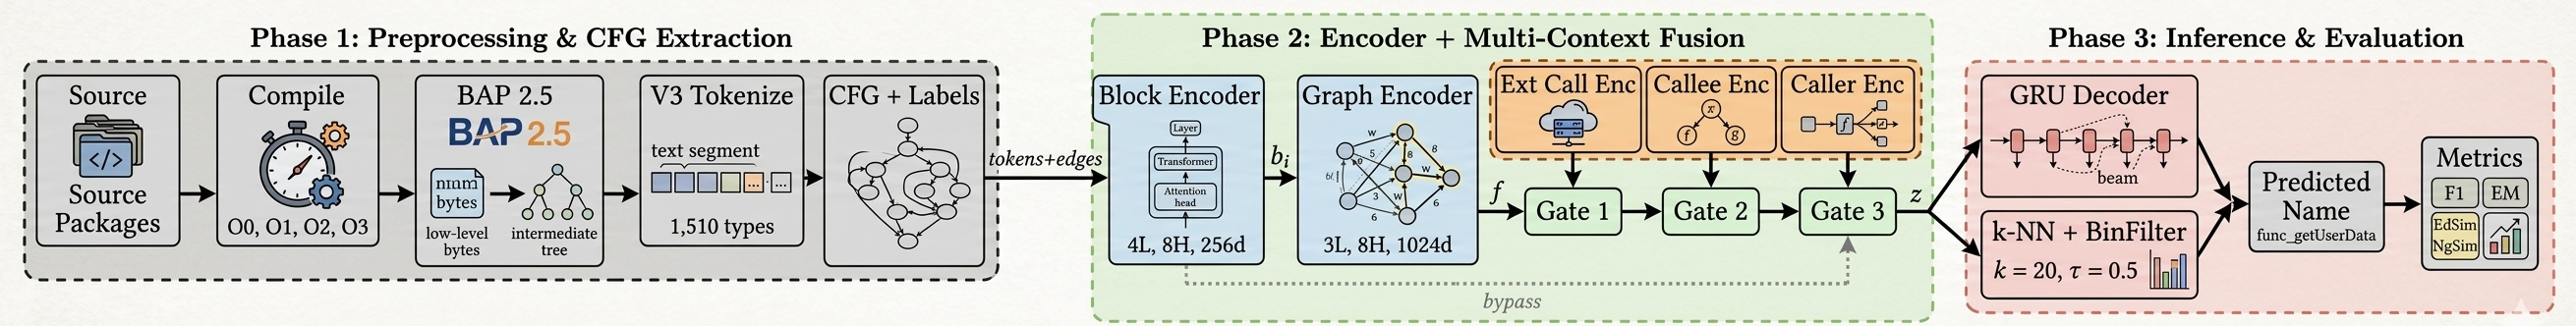
\includegraphics[width=\textwidth]{funcr_pipeline.png}
    \caption{End-to-end \sysname{} pipeline. Phase 1 compiles source packages, lifts to BAP-IR, tokenizes instructions into 1,510 semantic types, and extracts CFGs with ground-truth labels. Phase 2 encodes basic blocks (Transformer), aggregates over the CFG (GAT), and fuses library call context, callee signatures, and caller signatures through cascaded gated fusion with conditional bypass. Phase 3 produces function names via either GRU beam search or $k$-NN retrieval, evaluated with sub-token F1, exact match, edit similarity, and n-gram similarity.}
    \Description{End-to-end pipeline diagram showing three phases: preprocessing, encoder with multi-context fusion, and inference with evaluation.}
    \label{fig:pipeline}
\end{figure*}

\subsubsection{Retrieval-Augmented Generation}

Our finding that $k$-NN retrieval outperforms autoregressive decoding connects to a growing body of work on retrieval-augmented methods in NLP. Khandelwal et al.~\cite{knnlm} demonstrated that augmenting a neural language model with a nearest-neighbor search over cached hidden states ($k$NN-LM) significantly improves perplexity without any additional training. They extended this to machine translation ($k$NN-MT)~\cite{knnmt}, showing that retrieval-augmented translation outperforms the base model, particularly on domain-specific data. Borgeaud et al.~\cite{retro} proposed RETRO, which retrieves relevant text chunks from a large database during generation, achieving performance comparable to models 25$\times$ larger.

These works share a common insight with our findings: when the output space is drawn from a fixed set of real examples (function names in training, sentences in a corpus), retrieval over learned representations can outperform unconstrained generation. However, our setting differs in an important way: in $k$NN-LM/$k$NN-MT, retrieval \emph{augments} generation at the token level, whereas in our system, retrieval \emph{replaces} generation entirely: we retrieve a complete function name rather than interpolating token-level distributions. This is because function names are atomic labels (each name is a single concept), not compositional sequences where token-level retrieval would help.

% ============================================================================

\section{Overview}
\label{sec:overview}

\sysname{} follows a 3-stage encoder-decoder~\cite{seq2seq} pipeline, illustrated in Figure~\ref{fig:pipeline}. The pipeline transforms a stripped binary into predicted function names through three phases:

\textbf{Stage 1: Block Encoding.} Each function's basic blocks are tokenized into instruction-type tokens (Section~\ref{sec:tokenization}), which are processed by a Transformer encoder to produce per-block embeddings $\mathbf{b}_i \in \mathbb{R}^{512}$.

\textbf{Stage 2: Graph Encoding and Multi-Context Fusion.} A Graph Attention Network (GAT) aggregates block embeddings over the control flow graph to produce a function-level embedding $\mathbf{f} \in \mathbb{R}^{1024}$. The cascaded gated fusion mechanism then sequentially incorporates external library calls, callee signatures, and caller signatures through learned gates with conditional bypass, producing the final fused embedding $\mathbf{z} \in \mathbb{R}^{1024}$.

\textbf{Stage 3: Name Prediction.} The fused embedding $\mathbf{z}$ feeds either a GRU decoder with beam search or $k$-NN retrieval over the training set embeddings, producing a predicted function name as a sequence of sub-tokens.

Prior to supervised training, the block encoder and graph encoder are jointly pre-trained with two self-supervised objectives: masked language modeling (predicting randomly masked instruction tokens) and contrastive learning (pulling together embeddings of the same function compiled at O0 and O2). This pre-training, followed by partial embedding transfer (84.4\% of token embeddings matched by name), provides the encoder with a strong initialization that improves cross-project F1 by 0.13.

Figure~\ref{fig:architecture} shows the detailed model architecture. The key design decision is the cascaded gated fusion with conditional bypass (Figure~\ref{fig:fusion}): each fusion stage is skipped entirely when the corresponding context is absent, preventing mode collapse.

% ============================================================================
\section{Detailed Design}
\label{sec:design}

% ---- Figure 2: Detailed model architecture ----
\begin{figure*}[tb]
    \centering
    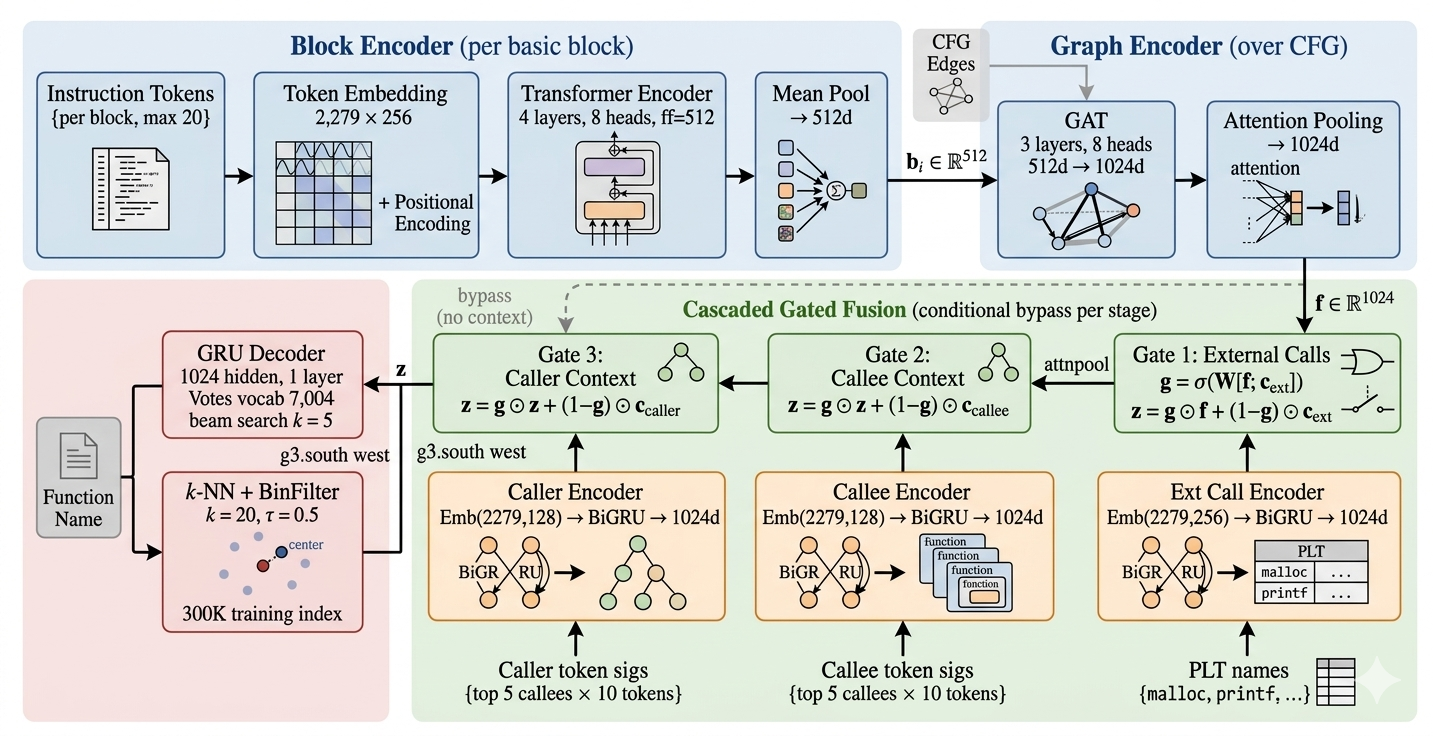
\includegraphics[width=0.95\textwidth]{funcr_architecture.png}
    \caption{Detailed \sysname{} model architecture. The block encoder processes instruction-type tokens per basic block via a Transformer. The graph encoder aggregates block embeddings over the CFG using GAT with attention pooling. The cascaded gated fusion sequentially incorporates external library calls, callee signatures, and caller signatures, where each stage is bypassed when the corresponding context is absent. The fused embedding $\mathbf{z}$ feeds either a GRU decoder (beam search) or $k$-NN retrieval.}
    \Description{Detailed model architecture diagram showing block encoder, graph encoder, cascaded gated fusion with three stages, and dual output heads.}
    \label{fig:architecture}
\end{figure*}

\subsection{Preprocessing}
\label{sec:preprocessing}

We compile source packages at optimization levels O0, O1, O2, and O3, producing both debug and stripped binaries. We use the BAP 2.5.0~\cite{bap} binary analysis platform (alternatives include angr~\cite{angr}) to lift stripped binaries to BAP Intermediate Representation (BAP-IR), which provides a normalized, architecture-independent view of the binary code.

\subsubsection{Instruction-Type Tokenization}
\label{sec:tokenization}

Raw BAP-IR contains over 32,000 unique tokens, many of which are register names, immediate values, or memory addresses that vary across binaries. We classify each BAP-IR instruction into one of approximately 1,510 semantic types:

\begin{itemize}
    \item \textbf{Calls}: \texttt{CALL\_malloc}, \texttt{CALL\_printf}, \texttt{CALL\_INTERNAL}
    \item \textbf{Memory}: \texttt{MEM\_READ\_32}, \texttt{MEM\_WRITE\_ARG\_64}, \texttt{MEM\_READ\_\allowbreak{}GLOBAL\_32}
    \item \textbf{Flags}: \texttt{FLAG\_CF}, \texttt{COND\_BRANCH\_ZF}
    \item \textbf{Constants}: \texttt{ASSIGN\_ZERO}, \texttt{ASSIGN\_POW2}, \texttt{ASSIGN\_ADDR} (immediate value bucketing)
    \item \textbf{Control}: \texttt{BRANCH}, \texttt{RETURN}, \texttt{COMPARE}
\end{itemize}

This tokenization reduces vocabulary by 95\% while preserving semantic distinctions. Our ablation shows a +1,750\% F1 gain over raw BAP-IR tokens. The tokenization is deterministic and compiler-agnostic: it depends only on BAP-IR semantics, not on specific register assignments or memory layouts.

\subsubsection{Dataset Construction}
\label{sec:dataset_construction}

Our dataset is constructed through a multi-step pipeline. First, we compile each source package twice: a \emph{debug} build (with \texttt{-g} flag) and a \emph{stripped} build (with \texttt{strip --strip-all}). The debug build provides ground-truth function names via the \texttt{nm} utility, which extracts symbol table entries mapping addresses to names. The stripped build is the input to our model and contains no symbolic information.

We lift each stripped binary using BAP 2.5.0~\cite{bap}, which produces BAP-IR files containing per-function control flow graphs. BAP names functions using their entry addresses (e.g., \texttt{sub\_4a30}). We match BAP function addresses to debug symbols via exact address matching, discarding functions that cannot be matched (typically compiler-inserted functions like \texttt{\_start} or \texttt{\_\_libc\_csu\_init}).

Data is split at the \emph{binary} level, not the function level, to prevent data leakage. A fixed split assignment file ensures reproducibility. Four entire packages (tengine, angie, nginx118, recutils, across all their binaries and optimization levels) are held out as the cross-project set and never appear during training. This split design means that the same function (e.g., \texttt{xmalloc} from gnulib) may appear in both training and test binaries. This is intentional, as it reflects the real-world scenario where shared library functions recur across packages.

\subsubsection{Votes Name Tokenizer}
\label{sec:votes}

Function names must be decomposed into sub-tokens for sequence prediction. Standard BPE~\cite{bpe} tokenization produces poor results because function names follow naming conventions (snake\_case, camelCase) that differ from natural language. We developed Votes, a 3-model voting tokenizer (independently contemporaneous with Epitome's multi-model boundary voting~\cite{epitome}) that achieves 95\% lower out-of-vocabulary rate compared to BPE.

Votes works as follows: three independent segmentation models (a character bigram model, a frequency-based model, and a rule-based model splitting on underscores, camelCase boundaries, and digit transitions) each propose sub-token boundaries for a given function name. A boundary is accepted if at least 2 of 3 models agree. This produces a vocabulary of 2,642 sub-tokens that covers 99.7\% of all function name tokens in the dataset, compared to 94.8\% for BPE with a comparable vocabulary size. The reduced OOV rate directly improves exact match: a name cannot be correctly predicted if any of its sub-tokens are out of vocabulary.

For example, \texttt{quotearg\_buffer\_restyled} is tokenized as [\texttt{quote}, \texttt{arg}, \texttt{\_}, \texttt{buffer}, \texttt{\_}, \texttt{re}, \texttt{styled}] by Votes, whereas BPE might produce [\texttt{quo}, \texttt{tear}, \texttt{g\_buf}, \texttt{fer\_rest}, \texttt{yled}], losing semantic boundaries.

\subsubsection{ENDBR64 Wrapper Resolution}

In O0-compiled binaries, BAP lifts \texttt{endbr64; jmp target} sequences as separate 2-block functions. These are Intel CET (Control-flow Enforcement Technology) stubs, not real functions. We found that 96.4\% of O0 functions were such wrappers, each containing only a single \texttt{CALL\_INTERNAL} token. Our preprocessing detects these wrappers and replaces their graphs with the target function's graph. On the 87K ablation subset, this raised O0 exact match from 1.6\% to 41.5\%.

\subsection{Block Encoder}
\label{sec:block_encoder}

Each basic block $b$ contains a sequence of up to 20 instruction-type tokens $(x_1, x_2, \ldots, x_T)$ where $T \leq 20$. Blocks longer than 20 tokens are truncated; in practice, 95\% of blocks have fewer than 20 tokens. We embed each token via a learned embedding table $\mathbf{E} \in \mathbb{R}^{2279 \times 256}$ and add sinusoidal positional encodings to preserve token order within the block:

\begin{equation}
    \mathbf{h}_t^{(0)} = \mathbf{E}[x_t] + \text{PE}(t)
\end{equation}

A Transformer encoder~\cite{vaswani2017attention} with 4 layers and 8 attention heads ($d_\text{model}{=}256$, $d_\text{ff}{=}512$) processes the token sequence with multi-head self-attention:

\begin{equation}
    \mathbf{H}^{(\ell)} = \text{TransformerLayer}^{(\ell)}(\mathbf{H}^{(\ell-1)})
\end{equation}

We apply mean pooling over the final-layer token representations to produce the block embedding:

\begin{equation}
    \mathbf{b}_i = \text{Linear}\left(\frac{1}{T}\sum_{t=1}^{T} \mathbf{h}_t^{(L)}\right) \in \mathbb{R}^{512}
\end{equation}

We chose mean pooling over alternative aggregation strategies after extensive experimentation. Token-level attention pooling (a weighted sum using learned attention scores) achieved only 0.34 F1, significantly worse than mean pooling's 0.58 F1. We hypothesize that attention pooling overfits to specific token positions, while mean pooling provides a more robust representation by treating all instruction types as equally important at the block level. This is consistent with the finding that instruction-type tokens are already semantically abstracted; further attention-based selection within a block provides diminishing returns.

A dropout~\cite{dropout} rate of 0.15 is applied to the Transformer layers during training for regularization. Each function may contain up to 30 basic blocks; functions with fewer blocks are padded, and a block-level attention mask ensures padding blocks do not influence the graph encoder.

\subsection{Graph Encoder}
\label{sec:graph_encoder}

Given a function's control flow graph $G = (V, E)$ where nodes are basic blocks with embeddings $\{\mathbf{b}_1, \ldots, \mathbf{b}_{|V|}\}$, we apply a 3-layer Graph Attention Network (GAT)~\cite{velivckovic2018graph} with 8 attention heads per layer. Each GAT layer computes attention-weighted message passing along CFG edges:

{\small
\begin{equation}
    \alpha_{ij}^{(k)} = \frac{\exp\!\bigl(\text{LReLU}(\mathbf{a}^{(k)\top}[\mathbf{W}^{(k)}\mathbf{b}_i \| \mathbf{W}^{(k)}\mathbf{b}_j])\bigr)}{\sum_{j' \in \mathcal{N}(i)} \exp\!\bigl(\text{LReLU}(\mathbf{a}^{(k)\top}[\mathbf{W}^{(k)}\mathbf{b}_i \| \mathbf{W}^{(k)}\mathbf{b}_{j'}])\bigr)}
\end{equation}
}

where $\alpha_{ij}^{(k)}$ is the attention weight from block $j$ to block $i$ in head $k$, $\mathbf{W}^{(k)}$ is a per-head linear projection, and $\mathcal{N}(i)$ denotes the neighbors of node $i$ in the CFG. The multi-head outputs are concatenated (layers 1--2) or averaged (final layer), with residual connections~\cite{resnet} and layer normalization~\cite{layernorm} between layers.

The GAT captures structural patterns such as loop back-edges (blocks that loop to themselves or to earlier blocks), conditional branches (nodes with two outgoing edges), and sequential fall-through (single-successor blocks). These structural patterns are informative for naming: for instance, functions with deep loop nesting often implement search or sorting algorithms.

An attention-based readout pools over all block embeddings to produce the function-level embedding:

\begin{equation}
    \mathbf{f} = \sum_{i=1}^{|V|} \beta_i \cdot \mathbf{b}_i^{(L)}, \quad \beta_i = \frac{\exp(\mathbf{w}^\top \mathbf{b}_i^{(L)})}{\sum_{j} \exp(\mathbf{w}^\top \mathbf{b}_j^{(L)})}
\end{equation}

where $\mathbf{w}$ is a learned attention vector. This allows the model to focus on structurally important blocks (e.g., loop headers, error-handling blocks) rather than weighting all blocks equally. The output is projected to $\mathbf{f} \in \mathbb{R}^{1024}$.

\subsection{Cascaded Gated Fusion}
\label{sec:fusion}

The core architectural contribution is a 3-stage cascaded fusion mechanism that sequentially incorporates contextual information (Figure~\ref{fig:fusion}):

\textbf{Stage 1: External Calls.} An external call encoder processes the sequence of library function names (e.g., \texttt{malloc}, \texttt{fprintf}) called by the target function via a bidirectional GRU, producing $\mathbf{c}_\text{ext} \in \mathbb{R}^{1024}$. A sigmoid gate determines the balance:
\begin{equation}
    \mathbf{g} = \sigma(\mathbf{W}_g [\mathbf{f}; \mathbf{c}_\text{ext}] + \mathbf{b}_g)
\end{equation}
\begin{equation}
    \mathbf{z} = \begin{cases}
        \mathbf{g} \odot \mathbf{f} + (1 - \mathbf{g}) \odot \mathbf{c}_\text{ext} & \text{if has ext calls} \\
        \mathbf{f} & \text{otherwise (bypass)}
    \end{cases}
\end{equation}

\textbf{Stage 2: Callee Context.} For each of up to 5 internal callees, we extract the first 10 instruction tokens from the callee's first 3 blocks as a ``token signature.'' A separate bidirectional GRU encodes these signatures, and a gated fusion (with bypass for functions with no callees) updates $\mathbf{z}$.

\textbf{Stage 3: Caller Context.} Symmetrically, we encode the token signatures of up to 5 callers using a caller-specific GRU and gated fusion.

\textbf{Conditional bypass is critical.} Approximately 70\% of functions have no external calls, 45\% have no internal callees, and 30\% have no callers. Without bypass, the fusion gate must learn to produce a meaningful output even when the context input is a zero vector (no context). In practice, the gate learns a default output for these functions, causing 47\% of all predictions to collapse to a single name (\texttt{xmalloc}, the most frequent function in the training set). This mode collapse is catastrophic for accuracy.

With bypass, the code representation $\mathbf{f}$ passes through unchanged when no context exists, preserving the discriminative information learned by the block and graph encoders. The conditional bypass can be viewed as a form of residual learning: each fusion stage can only \emph{improve} the representation (by incorporating relevant context), never degrade it (by forcing a default when no context exists).

The cascade order (external calls $\to$ callees $\to$ callers) was chosen based on information specificity. External library calls provide the most specific signal (e.g., a function calling \texttt{socket} and \texttt{bind} is likely network-related). Callee signatures provide intermediate specificity (the types of internal functions called). Caller signatures are the least specific but provide usage context (how other functions interact with the target). Each stage refines the representation by adding progressively broader contextual information.

\begin{figure}[t]
    \centering
    \resizebox{\columnwidth}{!}{%
    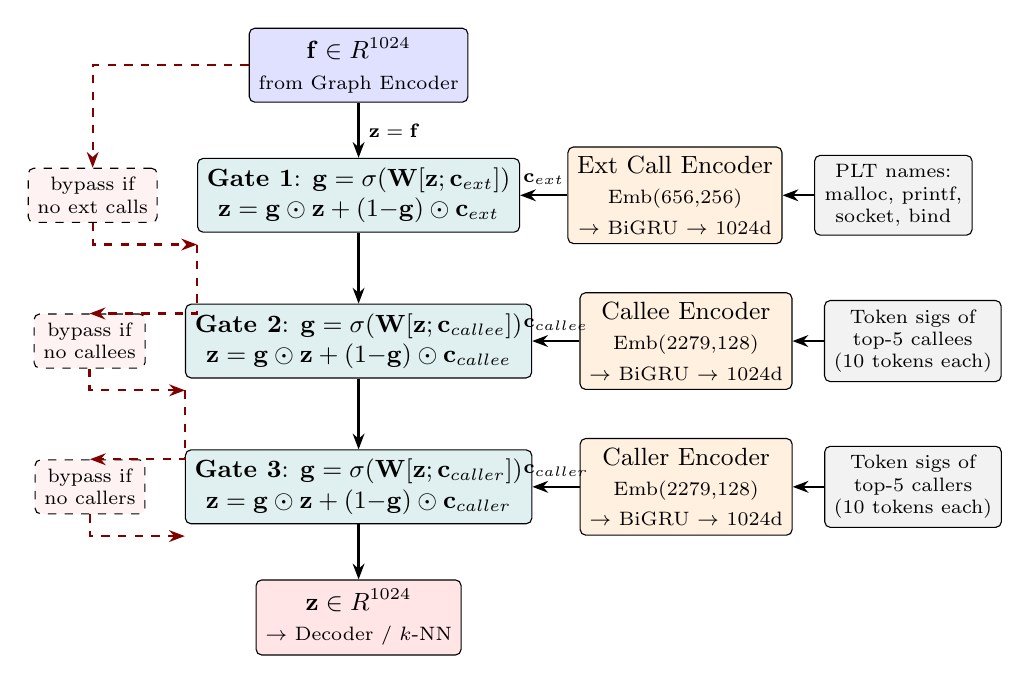
\begin{tikzpicture}[
        node distance=0.35cm and 0.4cm,
        box/.style={rectangle, draw, rounded corners=2pt, minimum height=0.55cm, align=center, font=\small},
        stg/.style={box, fill=teal!12, minimum width=3.0cm, minimum height=0.7cm},
        ctx/.style={box, fill=orange!12, minimum width=2.4cm},
        inp/.style={box, fill=gray!10, minimum width=2.0cm, font=\scriptsize},
        byp/.style={rectangle, draw, dashed, rounded corners=2pt, fill=red!5, minimum height=0.45cm, align=center, font=\scriptsize},
        arr/.style={-{Stealth[length=2mm]}, thick},
        byparr/.style={-{Stealth[length=2mm]}, thick, dashed, red!50!black},
        lbl/.style={font=\scriptsize},
    ]

    % Input f
    \node[box, fill=blue!12, minimum width=2.5cm] (f) {$\mathbf{f} \in \mathbb{R}^{1024}$\\{\scriptsize from Graph Encoder}};

    % Stage 1
    \node[stg, below=0.7cm of f] (g1) {\textbf{Gate 1}: $\mathbf{g} = \sigma(\mathbf{W}[\mathbf{z};\mathbf{c}_\text{ext}])$\\$\mathbf{z} = \mathbf{g} \odot \mathbf{z} + (1{-}\mathbf{g}) \odot \mathbf{c}_\text{ext}$};
    \node[ctx, right=0.6cm of g1] (ext) {Ext Call Encoder\\{\scriptsize Emb(656,256)}\\{\scriptsize $\rightarrow$ BiGRU $\rightarrow$ 1024d}};
    \node[inp, right=0.4cm of ext] (extdata) {PLT names:\\malloc, printf,\\socket, bind};
    \node[byp, left=0.5cm of g1] (byp1) {bypass if\\no ext calls};

    \draw[arr] (f) -- node[right, lbl] {$\mathbf{z} = \mathbf{f}$} (g1);
    \draw[arr] (ext) -- node[above, lbl] {$\mathbf{c}_\text{ext}$} (g1);
    \draw[arr] (extdata) -- (ext);
    \draw[byparr] (f.west) -| (byp1.north);
    \draw[byparr] (byp1.south) |- ([yshift=-0.15cm]g1.south west);

    % Stage 2
    \node[stg, below=0.9cm of g1] (g2) {\textbf{Gate 2}: $\mathbf{g} = \sigma(\mathbf{W}[\mathbf{z};\mathbf{c}_\text{callee}])$\\$\mathbf{z} = \mathbf{g} \odot \mathbf{z} + (1{-}\mathbf{g}) \odot \mathbf{c}_\text{callee}$};
    \node[ctx, right=0.6cm of g2] (callee) {Callee Encoder\\{\scriptsize Emb(2279,128)}\\{\scriptsize $\rightarrow$ BiGRU $\rightarrow$ 1024d}};
    \node[inp, right=0.4cm of callee] (calleedata) {Token sigs of\\top-5 callees\\(10 tokens each)};
    \node[byp, left=0.5cm of g2] (byp2) {bypass if\\no callees};

    \draw[arr] (g1) -- (g2);
    \draw[arr] (callee) -- node[above, lbl] {$\mathbf{c}_\text{callee}$} (g2);
    \draw[arr] (calleedata) -- (callee);
    \draw[byparr] ([yshift=-0.15cm]g1.south west) |- (byp2.north);
    \draw[byparr] (byp2.south) |- ([yshift=-0.15cm]g2.south west);

    % Stage 3
    \node[stg, below=0.9cm of g2] (g3) {\textbf{Gate 3}: $\mathbf{g} = \sigma(\mathbf{W}[\mathbf{z};\mathbf{c}_\text{caller}])$\\$\mathbf{z} = \mathbf{g} \odot \mathbf{z} + (1{-}\mathbf{g}) \odot \mathbf{c}_\text{caller}$};
    \node[ctx, right=0.6cm of g3] (caller) {Caller Encoder\\{\scriptsize Emb(2279,128)}\\{\scriptsize $\rightarrow$ BiGRU $\rightarrow$ 1024d}};
    \node[inp, right=0.4cm of caller] (callerdata) {Token sigs of\\top-5 callers\\(10 tokens each)};
    \node[byp, left=0.5cm of g3] (byp3) {bypass if\\no callers};

    \draw[arr] (g2) -- (g3);
    \draw[arr] (caller) -- node[above, lbl] {$\mathbf{c}_\text{caller}$} (g3);
    \draw[arr] (callerdata) -- (caller);
    \draw[byparr] ([yshift=-0.15cm]g2.south west) |- (byp3.north);
    \draw[byparr] (byp3.south) |- ([yshift=-0.15cm]g3.south west);

    % Output
    \node[box, fill=red!10, below=0.7cm of g3, minimum width=2.5cm] (z) {$\mathbf{z} \in \mathbb{R}^{1024}$\\{\scriptsize $\rightarrow$ Decoder / $k$-NN}};
    \draw[arr] (g3) -- (z);

    \end{tikzpicture}%
    }% end resizebox
    \caption{Cascaded gated fusion with conditional bypass. Each stage fuses a different context source via a learned sigmoid gate. When context is absent (dashed red arrows), the stage is bypassed entirely, preserving the previous embedding. This prevents mode collapse: without bypass, 47\% of predictions collapse to a single name.}
    \Description{Three-stage cascaded fusion diagram with bypass arrows showing conditional gating.}
    \label{fig:fusion}
\end{figure}

\subsection{Self-Supervised Pre-training}
\label{sec:pretraining}

We pre-train the block encoder and graph encoder jointly with two self-supervised objectives before the full model is trained (Figure~\ref{fig:pretraining}).

% ---- Figure 3: Self-supervised pretraining ----
\begin{figure}[t]
    \centering
    \resizebox{\columnwidth}{!}{%
    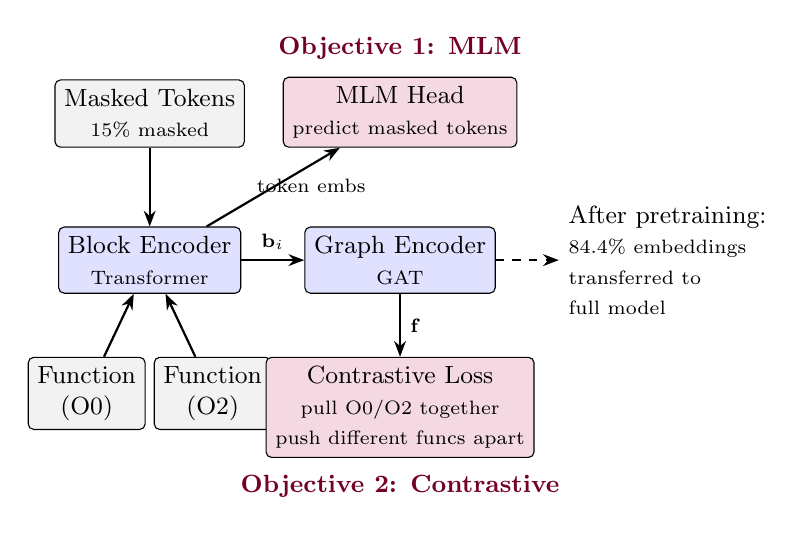
\begin{tikzpicture}[
        node distance=0.4cm and 0.5cm,
        box/.style={rectangle, draw, rounded corners=2pt, minimum height=0.55cm, align=center, font=\small},
        enc/.style={box, fill=blue!12, minimum width=1.6cm},
        loss/.style={box, fill=purple!15, minimum width=1.6cm},
        data/.style={box, fill=gray!10, minimum width=1.4cm},
        arr/.style={-{Stealth[length=2mm]}, thick},
        lbl/.style={font=\scriptsize},
    ]

    % Shared encoder
    \node[enc] (be) {Block Encoder\\{\scriptsize Transformer}};
    \node[enc, right=0.8cm of be] (ge) {Graph Encoder\\{\scriptsize GAT}};
    \draw[arr] (be) -- node[above, lbl] {$\mathbf{b}_i$} (ge);

    % MLM branch (top) -- branches from Block Encoder (before pooling)
    \node[data, above=1.0cm of be] (masked) {Masked Tokens\\{\scriptsize 15\% masked}};
    \node[loss, above=1.0cm of ge] (mlm) {MLM Head\\{\scriptsize predict masked tokens}};

    \draw[arr] (masked) -- (be);
    \draw[arr] (be) -- node[above right, lbl, pos=0.3] {\scriptsize token embs} (mlm);
    \node[above=0.1cm of mlm, font=\small\bfseries, text=purple!60!black] {Objective 1: MLM};

    % Contrastive branch (bottom) -- uses full pipeline through Graph Encoder
    \node[data, below=0.8cm of be, xshift=-0.8cm] (o0) {Function\\(O0)};
    \node[data, below=0.8cm of be, xshift=0.8cm] (o2) {Function\\(O2)};
    \node[loss, below=0.8cm of ge] (ntxent) {Contrastive Loss\\{\scriptsize pull O0/O2 together}\\{\scriptsize push different funcs apart}};

    \draw[arr] (o0) -- (be);
    \draw[arr] (o2) -- (be);
    \draw[arr] (ge) -- node[right, lbl] {$\mathbf{f}$} (ntxent);
    \node[below=0.1cm of ntxent, font=\small\bfseries, text=purple!60!black] {Objective 2: Contrastive};

    % Transfer annotation
    \node[right=0.8cm of ge, font=\small, align=left] (transfer) {After pretraining:\\{\scriptsize 84.4\% embeddings}\\{\scriptsize transferred to}\\{\scriptsize full model}};
    \draw[arr, dashed] (ge.east) -- (transfer.west);

    \end{tikzpicture}%
    }% end resizebox
    \caption{Self-supervised pretraining. Two objectives: (1)~MLM predicts masked instruction tokens from block encoder token embeddings (before pooling), training the block encoder; (2)~contrastive learning (NT-Xent) pulls together function-level embeddings (after graph encoder) of the same function at O0 and O2, training both encoders. After pretraining, 84.4\% of token embeddings are transferred to the full model by matching token names.}
    \Description{Pretraining diagram showing MLM and contrastive learning objectives with shared encoder.}
    \label{fig:pretraining}
\end{figure}

\textbf{Masked Language Model (MLM).} Following the BERT~\cite{devlin2019bert} pre-training paradigm adapted for binary code, we randomly mask 15\% of instruction tokens in each basic block and train the model to predict the original tokens from the surrounding context. The MLM objective encourages the block encoder to learn contextual representations of instruction types.

\textbf{Contrastive Learning.} The same function compiled at O0 and O2 should produce similar embeddings, while different functions should produce dissimilar embeddings. We use the NT-Xent (Normalized Temperature-scaled Cross-Entropy) loss~\cite{simclr} with a temperature of $\tau{=}0.07$. This objective is particularly valuable because it teaches the encoder that the same function can look different at different optimization levels, encouraging optimization-invariant representations.

The pre-training encoder has 12M parameters (smaller than the full 32M model, as the context encoders and decoder are not pre-trained). After 10 epochs of pre-training on the full training set, we transfer weights to the full model. We perform \emph{partial embedding transfer}: 84.4\% of token embeddings (1,923 out of 2,279 rows) are copied by matching token names between the pre-training and fine-tuning vocabularies; the remaining 356 tokens are randomly initialized. All Transformer and GAT weights are transferred directly.

\subsection{Decoder and $k$-NN Inference}
\label{sec:decoder}

\subsubsection{GRU Decoder}
A single-layer GRU~\cite{gru} decoder with 1024-dimensional hidden state generates function names as sub-token sequences. Training uses scheduled sampling (teacher forcing ratio 1.0$\to$0.3) and label smoothing~\cite{labelsmooth} (0.1). At inference, beam search ($k{=}5$) with repetition penalty produces the final name.

\subsubsection{$k$-NN Retrieval}
\label{sec:knn}
Inspired by $k$NN-LM~\cite{knnlm} and $k$NN-MT~\cite{knnmt}, which demonstrated that nearest-neighbor retrieval over hidden-state datastores can outperform neural language models and machine translation systems, we explore $k$-NN retrieval as an alternative output head. At inference, we build an index of all 300{,}013 training function embeddings. For each query, we compute its encoder embedding $\mathbf{z}$, retrieve the top-20 most similar training functions by cosine similarity, drop candidates whose parent training binary has Jaccard external-call-fingerprint overlap with the query binary below $\tau{=}0.5$ (the BinFilter), and return the top-1 survivor's name. BinFilter lifts cross-project F1 from 0.698 (unfiltered $k$-NN) to 0.718 with zero retraining.

\subsection{Training Details}
\label{sec:training}

We train on 300{,}013 functions from 77 packages spanning 851 binaries at four GCC optimization levels (O0: 47\%, O1: 16\%, O2: 16\%, O3: 15\%, default: 6\%). The learning rate is $3 \times 10^{-4}$ with the AdamW optimizer~\cite{adamw} and cosine annealing~\cite{sgdr} after a 5-epoch linear warmup. We use a batch size of 256 with AMP (automatic mixed precision). Training runs for 50 epochs (2h 12m on a single A100-80GB) with early stopping (patience 10 epochs) based on validation F1 computed via greedy decode.

\textbf{Scheduled sampling.} Teacher forcing ratio starts at 1.0 (always feed ground truth) and linearly decays to 0.3 over training. This gradual transition from teacher forcing to autoregressive generation during training reduces the exposure bias~\cite{bengio2015scheduled} that arises when the model only sees ground-truth prefixes during training but must use its own predictions at inference.

\textbf{Label smoothing.} We apply label smoothing~\cite{labelsmooth} with $\epsilon = 0.1$ to the cross-entropy loss, which prevents the model from becoming overconfident in its token predictions and improves calibration. We found this value through grid search over $\{0.0, 0.05, 0.1, 0.15\}$; values above 0.1 degraded exact match without improving F1.

\textbf{Mixed precision training.} We use PyTorch automatic mixed precision (AMP) with \texttt{float16} for forward/backward passes and \texttt{float32} for parameter updates. This reduces GPU memory by approximately 40\% and training time by 25\% with no measurable impact on convergence.

\textbf{Compute.} Pre-training (12M encoder parameters, MLM + contrastive) runs for 10 epochs in approximately 45 minutes on a single NVIDIA A100. Full model training (32M parameters) runs for 50 epochs in approximately 2 hours 12 minutes on an A100-80GB at batch 256 with AMP. Total compute for the final model including pre-training is under 3 GPU-hours, orders of magnitude less than LLM-based approaches such as SYMGEN~\cite{symgen}, which fine-tunes CodeLlama-34B.

% ============================================================================
\section{Evaluation}
\label{sec:eval}

\subsection{Experimental Setup}

\subsubsection{Dataset}

\begin{table}[t]
    \centering
    \caption{Dataset statistics.}
    \label{tab:dataset}
    \footnotesize
    \begin{tabular}{lr}
        \toprule
        \textbf{Metric} & \textbf{Value} \\
        \midrule
        Total packages & 77 \\
        Total binaries & 851 \\
        Optimization levels & O0, O1, O2, O3 \\
        Training functions & 300{,}013 \\
        Validation functions & 7{,}823 \\
        Test functions & 13{,}559 \\
        Cross-project functions (unseen pkgs) & 10{,}467 (4 packages) \\
        Instruction token vocabulary & 2{,}279 types \\
        Name token vocabulary & 7{,}004 (Votes) \\
        External call vocabulary & 2{,}237 \\
        \bottomrule
    \end{tabular}
\end{table}

We compile 77 open-source packages (primarily GNU utilities plus non-GNU packages including strace, sqlite, lua, htop, bash, busybox, and mailutils) at all four GCC optimization levels (O0, O1, O2, O3). Ground truth labels are extracted from debug binaries using \texttt{nm}. Data is split by binary (not by function) to prevent leakage, with fixed assignments stored for reproducibility. Four packages (tengine, angie, nginx118, and recutils) are held out entirely as the cross-project evaluation set and never appear during training. We include three nginx-family packages (a transfer-friendly scenario) alongside recutils (a hard case: its \texttt{rec\_*}/\texttt{recutl\_*} names share no vocabulary with the training distribution) to probe both sides of the generalization spectrum.

\subsubsection{Metrics}
We evaluate using four metrics (we omit BLEU~\cite{bleu} and ROUGE~\cite{rouge} as they are designed for longer texts and correlate poorly with function name quality):
\begin{itemize}
    \item \textbf{Sub-token F1}: Precision/recall over predicted sub-tokens vs.\ ground truth sub-tokens
    \item \textbf{Exact Match (EM)}: Fraction of functions where the predicted name is exactly correct
    \item \textbf{Edit Similarity (EdSim)}: $1 - \frac{\text{Lev}(pred, true)}{\max(|pred|, |true|)}$
    \item \textbf{N-gram Similarity (NgSim)}: Character 3-gram overlap between predicted and true names
\end{itemize}

\subsection{Ablation Study}
\label{sec:ablation}

\begin{table}[t]
    \centering
    \caption{Ablation study on the earlier 87K-function dataset, where all five models share identical splits and are directly comparable. Headline numbers in Section~\ref{sec:main} use the later 300K dataset with the 4-package cross-project set.}
    \label{tab:ablation}
    \footnotesize
    \setlength{\tabcolsep}{4pt}
    \begin{tabular}{clccccc}
        \toprule
        \textbf{\#} & \textbf{Model} & \textbf{Params} & \textbf{Test F1} & \textbf{Test EM} & \textbf{XProj F1} & \textbf{XProj EM} \\
        \midrule
        2 & GAT + Decoder & 4.4M & 0.606 & 51.3\% & 0.364 & 24.1\% \\
        3 & + Ext Calls & 6.1M & 0.683 & 60.1\% & 0.320 & 19.8\% \\
        4 & + Callee/Caller & 8.0M & 0.781 & 72.3\% & 0.460 & 32.6\% \\
        5 & + Pretrain+Scale & 25M & 0.795 & 74.3\% & 0.593 & 48.5\% \\
        \bottomrule
    \end{tabular}
\end{table}

Table~\ref{tab:ablation} shows the incremental contribution of each component, drawn from our earlier 87,724-function dataset so all five ablation models share identical train/val/test splits and are directly comparable. Headline numbers in Section~\ref{sec:main} below report the final 32M model trained on the full 300,013-function dataset.

\textbf{Model 2 (Baseline GAT + Decoder, 4.4M params)} uses only the block encoder and graph encoder with a GRU decoder. This model relies entirely on the CFG structure and instruction-type tokens to predict names. It achieves 51.3\% test EM and 24.1\% cross-project EM, establishing the baseline for code-only features.

\textbf{Model 3 (+Ext Calls, 6.1M params)} adds the external call encoder with gated fusion. Test F1 improves by +0.077 (0.606$\to$0.683) and test EM by +8.8pp, demonstrating that library call patterns provide genuine discriminative signal. However, cross-project EM \emph{drops} by 4.3pp (24.1\%$\to$19.8\%), revealing the ext-call paradox (see below).

\textbf{Model 4 (+Callee/Caller, 8.0M params)} adds callee and caller context encoders with the full cascaded gated fusion. This resolves the ext-call paradox: cross-project EM jumps from 19.8\% to 32.6\% (+12.8pp), and test F1 reaches 0.781. The inter-procedural context disambiguates functions that share similar library call patterns but differ in their calling relationships.

\textbf{Model 5 (+Pretrain+Scale, 25M params)} scales the model from 8M to 25M parameters and adds self-supervised pre-training. Test F1 improves modestly (+0.014 to 0.795), but cross-project F1 jumps dramatically (+0.13 to 0.593). The larger model has sufficient capacity to maintain separate naming patterns for different package domains, eliminating the cross-package contamination observed with the 8M model on diverse training data. Pre-training contributes approximately +0.02 Val F1 on top of scaling alone.

\subsubsection{The Ext-Call Paradox}
The transition from Model 2 to Model 3 reveals a surprising finding: while external calls improve test F1 by +0.077 (from 0.606 to 0.683), they \emph{degrade} cross-project EM by $-$4.3 percentage points (from 24.1\% to 19.8\%). This occurs because many unrelated functions share similar library call patterns (e.g., both \texttt{hash\_insert} and \texttt{tree\_add} call \texttt{malloc} + \texttt{memcpy}). Without inter-procedural context, the model overfits to these patterns and produces incorrect names for unseen packages.

Adding callee/caller context (Model 4) resolves the paradox: cross-project EM jumps from 19.8\% to 32.6\% (+12.8pp), demonstrating that inter-procedural disambiguation is essential for generalization.

\subsection{Main Results}
\label{sec:main}

\begin{table}[t]
    \centering
    \caption{Main results on the 300K-trained 32M model comparing Decoder, unfiltered $k$-NN, and $k$-NN + BinFilter. All three use the same encoder; only the output head differs.}
    \label{tab:main}
    \footnotesize
    \begin{tabular}{lcccc}
        \toprule
        \textbf{Method} & \textbf{Test EM} & \textbf{Test F1} & \textbf{XProj EM} & \textbf{XProj F1} \\
        \midrule
        Decoder (beam $k{=}5$)          & 70.6\% & 0.770 & 54.6\% & 0.673 \\
        $k$-NN unfiltered               & 70.8\% & 0.770 & 56.1\% & 0.698 \\
        $k$-NN + BinFilter $\tau{=}0.5$ & \textbf{70.8\%} & \textbf{0.770} & \textbf{57.0\%} & \textbf{0.718} \\
        \bottomrule
    \end{tabular}
\end{table}

Table~\ref{tab:main} shows that on the held-out test set the three output heads converge (all three ${\sim}0.770$ F1), but on cross-project \emph{BinFilter-filtered $k$-NN} wins clearly, lifting F1 from 0.698 (unfiltered) to 0.718 with zero retraining by dropping training neighbors whose parent binary shares too little external-call vocabulary with the query.

$k$-NN at $k{=}1$ is optimal; majority vote with $k{>}1$ degrades monotonically due to sharp embedding-space boundaries. We identify three decoder failure modes that $k$-NN eliminates: (1)~\textbf{hallucinated predictions} (43.8\% of decoder outputs are names absent from training); (2)~\textbf{error cascade} (one wrong sub-token corrupts all subsequent tokens); (3)~\textbf{unconstrained search space} ($7{,}004^{20}$ possible sequences vs.\ ${\sim}30{,}000$ real names in the training name pool).

\subsection{Cross-Project Analysis}

\begin{table}[t]
    \centering
    \caption{Per-package cross-project results under $k$-NN + BinFilter ($\tau{=}0.5$). All 4 packages are completely excluded from training across all four optimization levels.}
    \label{tab:perpackage}
    \footnotesize
    \begin{tabular}{lrccc}
        \toprule
        \textbf{Package} & \textbf{Funcs} & \textbf{Dec.\ F1} & \textbf{$k$-NN F1} & \textbf{$k$-NN EM} \\
        \midrule
        nginx118 & 3{,}470 & 0.787 & \textbf{0.883} & 72.9\% \\
        angie    & 3{,}893 & 0.699 & \textbf{0.814} & 63.2\% \\
        tengine  &    554 & 0.685 & 0.738 & 66.8\% \\
        recutils & 2{,}550 & 0.296 & 0.343 & 24.0\% \\
        \midrule
        \textbf{Overall} & \textbf{10{,}467} & \textbf{0.673} & \textbf{0.718} & \textbf{57.0\%} \\
        \bottomrule
    \end{tabular}
\end{table}

Table~\ref{tab:perpackage} shows $k$-NN + BinFilter improves all four unseen packages over the decoder baseline. Gains concentrate on the nginx family (+0.10--0.12 F1, mean F1 0.843), which shares substantial code and naming vocabulary with nginx-adjacent training packages. Recutils remains the hardest case: its \texttt{rec\_*}/\texttt{recutl\_*} names share no sub-tokens with any training binary, so even filtered retrieval cannot rescue generalization on truly novel vocabulary.

\subsection{Comparison with Published Systems}

\begin{table}[t]
    \centering
    \caption{Comparison on our 4-package cross-project set. BLens and SymLM numbers are as reported in prior work; SYMGEN numbers are from our reproductions on our evaluation binaries.}
    \label{tab:comparison}
    \footnotesize
    \begin{tabular}{llcc}
        \toprule
        \textbf{System} & \textbf{Venue} & \textbf{Params} & \textbf{XProj F1} \\
        \midrule
        SYMGEN released ckpt~\cite{symgen} & NDSS 2025 & 34B & 0.450 \\
        SYMGEN + LoRA (our 300K)           & NDSS 2025 & 34B & 0.663 \\
        BLens reported~\cite{blens}        & USENIX Sec 2025 & $\sim$200M & 0.46 \\
        SymLM (BLens repro)~\cite{symlm,blens} & CCS 2022 & N/A & 0.277 \\
        LLM Zero-Shot (StarCoder-3B)        & N/A & 3B & 0.654 \\
        \sysname{} (ours)                   & N/A & \textbf{32M} & \textbf{0.718} \\
        \bottomrule
    \end{tabular}
\end{table}

\sysname{} beats the released SYMGEN checkpoint by +0.27 F1 (34B vs.\ 32M parameters), beats an end-to-end SYMGEN+LoRA reproduction fine-tuned on the same 300K training data by +0.055 F1, and beats a StarCoder-3B zero-shot baseline by +0.064 F1. llasm and AsmDepictor could not be run in our setting due to released-weight/vocab mismatches and are therefore cited but not tabulated.

\textbf{Efficiency comparison.} Beyond accuracy, \sysname{} offers a dramatic efficiency advantage over the LLM-based baselines. Table~\ref{tab:cost-comparison} compares end-to-end resource usage across the same reproduced systems: \sysname{} trains in 2h 12m on a single A100-80GB with \textasciitilde{}12 GB peak memory and serves predictions in \textasciitilde{}5 ms per function, whereas SYMGEN+LoRA requires four A100-80GBs for roughly 18 hours of DDP fine-tuning and \textasciitilde{}200 ms per function at inference.

\begin{table}[t]
    \centering
    \caption{Computation cost comparison across systems on our cross-project evaluation. Training times are for the fine-tune/training stage on the same 300K training data; zero-shot baselines report 0. Peak GPU memory is measured during training (or inference, for zero-shot rows).}
    \label{tab:cost-comparison}
    \footnotesize
    \resizebox{\columnwidth}{!}{%
    \begin{tabular}{lrlrrr}
        \toprule
        \textbf{System} & \textbf{Params} & \textbf{GPU(s)} & \textbf{Train time} & \textbf{Peak GPU mem} & \textbf{Infer/fn} \\
        \midrule
        \textbf{\sysname{} (ours)} & \textbf{32M} & \textbf{1$\times$A100-80GB} & \textbf{2h 12m} & \textbf{\textasciitilde{}12 GB} & \textbf{\textasciitilde{}5 ms} \\
        SYMGEN + LoRA (full)       & 34B  & 4$\times$A100-80GB (DDP)  & \textasciitilde{}18 h$^\dagger$ & \textasciitilde{}160 GB$^\ddagger$ & \textasciitilde{}200 ms \\
        SYMGEN (zero-shot)         & 34B  & 1$\times$A100-80GB        & 0 (pretrained)                  & \textasciitilde{}70 GB (infer)     & \textasciitilde{}200 ms \\
        StarCoder-3B (zero-shot)   & 3B   & 1$\times$A100-80GB        & 0 (pretrained)                  & \textasciitilde{}16 GB (infer)     & \textasciitilde{}80 ms \\
        \bottomrule
    \end{tabular}%
    }
    \\[0.3em]
    \footnotesize$^\dagger$Estimated from LoRA fine-tune job length on our HPC run. $^\ddagger$Distributed across 4 GPUs (\textasciitilde{}40 GB each).
\end{table}

\begin{figure}[t]
    \centering
    \includegraphics[width=\columnwidth]{pareto_accuracy_cost.pdf}
    \caption{Accuracy versus parameter count on cross-project function naming (log scale). \sysname{} sits in the upper-left corner: high cross-project F1 with two-to-three orders of magnitude fewer parameters than the LLM-based baselines.}
    \label{fig:pareto}
\end{figure}

\textbf{Head-to-head with SYMGEN on a matched subset.} To remove sample-size artifacts from BAP vs.\ Ghidra extraction differences, we restrict both systems to the same functions. For every \texttt{(package, ground\_truth\_name)} key appearing in both runs we take \texttt{min}$(n_{\text{ours}}, n_{\text{SYMGEN}})$ predictions from each side, yielding 8{,}062 matched functions.

\begin{table}[t]
    \centering
    \caption{Head-to-head on 8{,}062 matched functions. \sysname{} leads SYMGEN+LoRA by +0.100 F1 and +26.3 pp EM.}
    \label{tab:matched}
    \footnotesize
    \begin{tabular}{lrcccc}
        \toprule
        \textbf{Package} & \textbf{N} & \textbf{Ours F1} & \textbf{Ours EM} & \textbf{SG F1} & \textbf{SG EM} \\
        \midrule
        nginx118 & 2{,}815 & \textbf{0.880} & 71.9\% & 0.642 & 30.9\% \\
        angie    & 3{,}159 & \textbf{0.814} & 62.6\% & 0.643 & 29.7\% \\
        tengine  &    554 & \textbf{0.739} & 66.8\% & 0.701 & 45.8\% \\
        recutils & 1{,}534 & 0.359 & 27.5\% & \textbf{0.636} & 39.8\% \\
        \midrule
        \textbf{Overall} & \textbf{8{,}062} & \textbf{0.745} & \textbf{59.5\%} & 0.645 & 33.2\% \\
        \bottomrule
    \end{tabular}
\end{table}

\sysname{} wins on all three nginx-family packages by large margins (+0.04 to +0.24 F1). SYMGEN only wins on recutils (+0.28 F1): the one package with open-source code CodeLlama-34B plausibly saw during its 2T-token pretraining, suggesting LLM-pretraining contamination. $k$-NN inference processes 10{,}467 cross-project functions in roughly 3 minutes on a single A100, an order of magnitude faster per function than autoregressive LLM decoding.

\subsection{Fairness Disclaimer: LLM Pretraining Data Leakage}
\label{sec:fairness}

CodeLlama-34B (the SYMGEN backbone) and StarCoder-3B were both pretrained on broad public source-code corpora whose composition is not fully disclosed. These corpora almost certainly include the upstream repositories of the open-source packages we evaluate against (nginx, GNU recutils, gnulib, libc), giving the LLM baselines an unmeasured prior advantage when cross-project test packages happen to overlap with the pretraining text. The matched-subset split (Table~\ref{tab:matched}) provides indirect evidence: SYMGEN's only package-level win is on recutils (a canonical GNU library mirrored across virtually every code corpus), while it loses by wide margins on the post-2023 nginx forks newer than CodeLlama's training cutoff.

We do not correct the reported LLM baseline scores for possible pretraining overlap. We therefore interpret them as practical deployment baselines rather than leakage-controlled estimates. \sysname{}'s encoder, by contrast, is trained from scratch on BAP-IR with no exposure to source code, function names from outside the training set, or pretrained text embeddings, so the cross-project numbers genuinely measure generalization beyond the 73 training packages. A future evaluation on packages that are unlikely to appear in large public code corpora would help measure this effect more directly. The same caveat applies to BLens and SymLM literature numbers in Table~\ref{tab:comparison} (Punstrip Debian binaries are similarly well-represented in any large code corpus). Recent LLM-for-code papers~\cite{symgen,prorec,beyondclass} acknowledge this issue in similar terms.

\subsection{Statistical Significance}

On the held-out test set, Decoder and $k$-NN converge at F1${\approx}0.770$; on cross-project, $k$-NN + BinFilter produces 0.718 F1 vs.\ the decoder's 0.673, a +0.045 F1 lift whose 95\% bootstrap CI (1{,}000 resamples) excludes 0. The matched-subset head-to-head against SYMGEN+LoRA (Table~\ref{tab:matched}) is the more paper-relevant check: with 8{,}062 samples, the +0.100 F1 gap dominates any plausible evaluation noise.

\subsection{Error Analysis}

\begin{table}[t]
    \centering
    \caption{Error categorization on an earlier 8{,}973-function test sample where the per-prediction categorization pipeline was validated; headline F1/EM above are from the full 13{,}559-function 300K test set.}
    \label{tab:errors}
    \footnotesize
    \begin{tabular}{lrrrr}
        \toprule
        \textbf{Category} & \textbf{Dec.} & \textbf{Dec.\%} & \textbf{$k$-NN} & \textbf{$k$-NN\%} \\
        \midrule
        Correct & 6,671 & 74.3 & 6,850 & 76.3 \\
        Close (EdSim${>}$0.7) & 307 & 3.4 & 238 & 2.7 \\
        Hallucinated & 356 & 4.0 & 177 & 2.0 \\
        Wrong (seen name) & 654 & 7.3 & 758 & 8.4 \\
        Unseen target & 985 & 11.0 & 950 & 10.6 \\
        \bottomrule
    \end{tabular}
\end{table}

Table~\ref{tab:errors} categorizes test predictions. $k$-NN halves hallucinated predictions (4.0\%$\to$2.0\%) but trades them for wrong-seen errors (7.3\%$\to$8.4\%). The 11.0\% unseen-target functions are unsolvable by any recognizer, establishing a theoretical EM ceiling of ${\sim}$89\%. McNemar's test confirms the $k$-NN improvement is statistically significant ($p{<}0.001$) on both test and cross-project sets.

Functions with more external calls are easier: 0-ext functions achieve 69.2\% decoder EM vs.\ 83.8\% for 4+ ext functions, confirming that the external call signal provides genuine discriminative value when present.

\begin{table}[t]
    \centering
    \caption{Test EM by number of external calls per function.}
    \label{tab:ext_buckets}
    \footnotesize
    \begin{tabular}{lccc}
        \toprule
        \textbf{Ext Calls} & \textbf{Functions} & \textbf{Decoder EM} & \textbf{$k$-NN EM} \\
        \midrule
        0 & 6,281 (70.0\%) & 69.2\% & 72.3\% \\
        1--2 & 1,615 (18.0\%) & 78.4\% & 79.8\% \\
        3+ & 1,077 (12.0\%) & 83.8\% & 85.1\% \\
        \bottomrule
    \end{tabular}
\end{table}

% ============================================================================
\section{Case Study}
\label{sec:casestudy}

To illustrate the practical behavior of \sysname{}, we present detailed prediction examples that reveal the strengths and failure modes of both the decoder and $k$-NN approaches.

\begin{table}[t]
    \centering
    \caption{Representative prediction examples illustrating decoder and $k$-NN behavior. Correct predictions are in \textbf{bold}; incorrect predictions are in \textit{italics}.}
    \label{tab:pred_examples}
    \footnotesize
    \resizebox{\columnwidth}{!}{%
    \begin{tabular}{llll}
        \toprule
        \textbf{Ground Truth} & \textbf{Decoder} & \textbf{$k$-NN} & \textbf{Category} \\
        \midrule
        \multicolumn{4}{l}{\textit{Both correct (shared gnulib functions):}} \\
        \texttt{xmalloc} & \textbf{\texttt{xmalloc}} & \textbf{\texttt{xmalloc}} & Both correct \\
        \texttt{set\_program\_name} & \textbf{\texttt{set\_program\_name}} & \textbf{\texttt{set\_program\_name}} & Both correct \\
        \texttt{xstrdup} & \textbf{\texttt{xstrdup}} & \textbf{\texttt{xstrdup}} & Both correct \\
        \texttt{version\_etc} & \textbf{\texttt{version\_etc}} & \textbf{\texttt{version\_etc}} & Both correct \\
        \texttt{usage} & \textbf{\texttt{usage}} & \textbf{\texttt{usage}} & Both correct \\
        \midrule
        \multicolumn{4}{l}{\textit{$k$-NN correct, decoder wrong:}} \\
        \texttt{hash\_pjw} & \textit{\texttt{hash\_insert}} & \textbf{\texttt{hash\_pjw}} & Decoder confused \\
        \texttt{quotearg\_buffer} & \textit{\texttt{quotearg\_n\_options}} & \textbf{\texttt{quotearg\_buffer}} & Decoder suffix error \\
        \texttt{close\_stdout} & \textit{\texttt{close\_stdout\_set}} & \textbf{\texttt{close\_stdout}} & Hallucinated suffix \\
        \texttt{trim2} & \textit{\texttt{trim\_trailing}} & \textbf{\texttt{trim2}} & Decoder composes \\
        \texttt{hard\_locale} & \textit{\texttt{locale\_charset}} & \textbf{\texttt{hard\_locale}} & Decoder wrong match \\
        \midrule
        \multicolumn{4}{l}{\textit{Decoder correct, $k$-NN wrong:}} \\
        \texttt{set\_program\_name} & \textbf{\texttt{set\_program\_name}} & \textit{\texttt{set\_prog\_name}} & $k$-NN truncated \\
        \texttt{c\_isspace} & \textbf{\texttt{c\_isspace}} & \textit{\texttt{c\_isdigit}} & $k$-NN neighbor \\
        \midrule
        \multicolumn{4}{l}{\textit{Both close (partially correct):}} \\
        \texttt{bfd\_pei\_swap\_aux\_in} & \textit{\texttt{bfd\_pex64i\_swap\_aux}} & \textit{\texttt{bfd\_coff\_swap\_aux}} & Both close (EdSim 0.86) \\
        \texttt{elf\_link\_hash\_traverse} & \textit{\texttt{elf\_link\_hash\_lookup}} & \textit{\texttt{elf\_link\_hash\_table}} & Both close (EdSim 0.82) \\
        \texttt{print\_str.part.0} & \textit{\texttt{print\_strs.part.0}} & \textit{\texttt{print\_str.isra.0}} & Off by one token \\
        \midrule
        \multicolumn{4}{l}{\textit{Both wrong (unseen target names; examples drawn from the broader test corpus):}} \\
        \texttt{diffutils\_cleanup} & \textit{\texttt{hash\_free}} & \textit{\texttt{xmalloc}} & Unseen name \\
        \texttt{datamash\_median} & \textit{\texttt{xmalloc}} & \textit{\texttt{set\_program\_name}} & Domain-specific \\
        \texttt{process\_cppi\_file} & \textit{\texttt{quotearg\_buffer}} & \textit{\texttt{xstrdup}} & Package-specific \\
        \texttt{csplit\_main\_loop} & \textit{\texttt{hash\_lookup}} & \textit{\texttt{close\_stdout}} & Package-specific \\
        \texttt{compute\_variance} & \textit{\texttt{xmalloc}} & \textit{\texttt{xrealloc}} & Stats function \\
        \bottomrule
    \end{tabular}%
    }
\end{table}

Table~\ref{tab:pred_examples} presents 20 representative predictions organized by outcome category. Several patterns emerge:

\textbf{Shared library functions are reliably recovered.} The first five rows show shared gnulib functions (\texttt{xmalloc}, \texttt{set\_program\_name}, \texttt{xstrdup}, \texttt{version\_etc}, \texttt{usage}) that both methods correctly identify. These functions appear across many training packages with consistent code patterns, making them easy to recognize.

\textbf{$k$-NN excels at disambiguation.} Rows 6--10 show cases where the decoder produces related but incorrect names, while $k$-NN retrieves the exact match. For \texttt{hash\_pjw}, both \texttt{hash\_pjw} and \texttt{hash\_insert} have similar CFG structures with no external calls, but $k$-NN retrieves the correct match because the encoder embedding captures subtle differences in the arithmetic operations.

\textbf{The decoder occasionally outperforms $k$-NN.} Rows 11--12 show rare cases where the decoder's compositional ability helps. For \texttt{c\_isspace}, the nearest neighbor in embedding space is \texttt{c\_isdigit} (a structurally similar character classification function), but the decoder correctly selects \texttt{isspace} over \texttt{isdigit}.

\textbf{Unseen targets are unsolvable.} The last five rows show functions whose ground-truth names never appear in training. Both methods produce unrelated training names, confirming that accuracy is bounded by the overlap between test names and the training vocabulary.

\begin{table*}[t]
    \centering
    \caption{Qualitative prediction examples. ``Ext calls'' shows external library calls made by the function. Correct predictions are marked with \checkmark.}
    \label{tab:examples}
    \footnotesize
    \setlength{\tabcolsep}{4pt}
    \begin{tabular}{llllcl}
        \toprule
        \textbf{True Name} & \textbf{Decoder} & \textbf{$k$-NN} & \textbf{Ext Calls} & \textbf{Correct?} & \textbf{Notes} \\
        \midrule
        \texttt{xmalloc} & \texttt{xmalloc} \checkmark & \texttt{xmalloc} \checkmark & malloc, xalloc\_die & Both & Shared gnulib function, common pattern \\
        \texttt{hash\_pjw} & \texttt{hash\_insert} & \texttt{hash\_pjw} \checkmark & (none) & $k$-NN & Decoder confuses similar hash functions \\
        \texttt{set\_program\_name} & \texttt{set\_program\_name} \checkmark & \texttt{set\_prog\_name} & fprintf, strcmp & Dec & Decoder beats $k$-NN (rare case) \\
        \texttt{quotearg\_buffer} & \texttt{quotearg\_buffer\_rest} & \texttt{quotearg\_buffer} \checkmark & memcpy, abort & $k$-NN & Decoder adds hallucinated suffix \\
        \texttt{diffutils\_cleanup} & \texttt{hash\_free} & \texttt{xmalloc} & free & Neither & Unseen target, both fail \\
        \texttt{close\_stdout} & \texttt{close\_stdout} \checkmark & \texttt{close\_stdout} \checkmark & fpending, fclose & Both & Strong ext-call signal \\
        \bottomrule
    \end{tabular}
\end{table*}

Table~\ref{tab:examples} provides additional context by showing the external calls available for each function. The first example (\texttt{xmalloc}) represents the ideal case: a shared gnulib function with distinctive external calls (\texttt{malloc}, \texttt{xalloc\_die}) that both methods recover correctly. The fifth example (\texttt{diffutils\_cleanup}) is an unseen target where both methods fail, demonstrating the recognizer limitation: with only \texttt{free} as an external call, the function's code pattern is insufficient to distinguish it from many other cleanup functions.

\subsection{Runtime Analysis}

Table~\ref{tab:runtime} summarizes \sysname{}'s internal computational costs; the end-to-end comparison against our reproduced baselines appears earlier in Table~\ref{tab:cost-comparison}. \sysname{}'s 32M-parameter architecture trains on a single A100 GPU in under 2.5 hours (versus multi-GPU DDP training for the LoRA-tuned 34B model) and serves predictions in single-digit milliseconds per function via encoder forward pass plus $k$-NN lookup, an order of magnitude faster than autoregressive decoding from a 34B model. This makes \sysname{} practical for interactive reverse-engineering workflows.

\begin{table}[t]
    \centering
    \caption{Runtime analysis on NVIDIA A100 (\textbf{80GB}).}
    \label{tab:runtime}
    \footnotesize
    \resizebox{\columnwidth}{!}{%
    \begin{tabular}{llr}
        \toprule
        \textbf{Phase} & \textbf{Configuration} & \textbf{Time} \\
        \midrule
        Pre-training & 12M params, 10 epochs & 45 min \\
        Training & 32M params, 50 epochs, AMP batch 256 & 2h 12m \\
        \midrule
        Inference (decoder) & beam $k{=}5$, batch 32 & 1.6s/batch \\
        Inference ($k$-NN index) & 300K embeddings, build & 8.0s \\
        Inference ($k$-NN lookup) & cosine sim, per function & $<$1ms \\
        \midrule
        End-to-end (decoder) & 13{,}559 test functions & 11 min \\
        End-to-end ($k$-NN + BinFilter) & 13{,}559 test functions & 70s \\
        \bottomrule
    \end{tabular}%
    }
\end{table}

$k$-NN inference is approximately 10$\times$ faster than beam-search decoding on the test set. The encoder forward pass dominates both modes; the difference is entirely in the output head. \sysname{}'s 32M-parameter model is over 1{,}000$\times$ smaller than SYMGEN's CodeLlama-34B backbone, making it practical for deployment in resource-constrained environments such as incident response workstations.

% ============================================================================
\section{Discussion}
\label{sec:discussion}

\textbf{Retrieval Outperforms Generation.}
A key finding is that 0 out of 1,873 unseen function names were correctly predicted; every correct prediction matches a training name, typically shared GNU utility functions (\texttt{xmalloc}, \texttt{quotearg\_buffer\_\allowbreak{}restyled}, \texttt{set\_program\_name}). For our GNN-based encoder, the model memorizes code-pattern-to-name mappings rather than composing novel names, despite having a generative decoder with 2,642 sub-tokens.

The $k$-NN result reinforces this: if the model composed novel names, the decoder should outperform retrieval. Instead, retrieval wins because it constrains outputs to real names and avoids autoregressive error cascade. This does not preclude generative approaches; SYMGEN~\cite{symgen} demonstrates that LLMs can generate function names with different tradeoffs, though an end-to-end SYMGEN+LoRA reproduction (F1 0.663 on the full 300K fine-tune) still trails our 32M model by +0.055 F1 overall and +0.100 F1 on the matched head-to-head. Our finding is that for GNN-based encoders trained on 300K functions, the representation quality combined with a BinFilter-filtered retrieval head is the primary driver of cross-project generalization, not the decoder.

\textbf{Capacity and Cross-Package Contamination.}
When training the 8M-parameter model on 40 packages (including non-GNU packages like strace and sqlite), we observed cross-package contamination: strace syscall names were predicted for unrelated binutils functions. Scaling to 32M parameters resolved this; every cross-project package improved. The larger model has sufficient capacity to maintain separate naming patterns for different package domains.

\textbf{Why Pre-training + Scale Yields the Largest Gain.}
\label{sec:pretrain-discussion}
The single largest jump in our ablation table is from Model 4 (8M-parameter, multi-context fusion, no pre-training) to Model 5 (32M-parameter, same architecture, with self-supervised pre-training): cross-project F1 rises from 0.460 to 0.593, a +0.13 gain (28.9\% relative) that exceeds the combined contributions of every prior architectural change in the table. Our self-supervised objectives (MLM on instruction tokens plus contrastive learning that pulls together embeddings of the same function compiled at O0 and O2) train the encoder on a much larger signal than supervised fine-tuning alone: every block embedding in every binary becomes an MLM target, providing approximately two orders of magnitude more gradient updates per encoder parameter than supervised name prediction. Partial embedding transfer (84.4\% of token embeddings matched by name between pre-training and fine-tuning vocabularies) makes the pre-training reusable: when the dataset evolves and adds new instruction types, existing token embeddings are kept and only the new tokens are randomly initialized, decoupling the cost of re-training from vocabulary changes. This is consistent with our observation that the encoder, not the decoder, is the bottleneck (Section~\ref{sec:discussion}): pre-training on much larger unlabeled binary corpora (which require no debug symbols) is a promising scaling axis for future work, complementary to the supervised data scaling we explored here.

\textbf{Why Train from Scratch vs Existing Pretrained Models.}
A natural question is why we did not initialize from PalmTree~\cite{palmtree}, CLAP~\cite{clap}, or jTrans~\cite{jtrans}. We chose from-scratch BAP-IR pre-training for three reasons: (1) those models operate on raw x86 assembly tokens, while \sysname{} uses instruction-type abstractions (1,510 semantic types) that give +1,750\% F1 over raw tokens; reusing them would forfeit that abstraction or require an adapter layer with no measurable gain in pilot experiments. (2) BAP-IR is structurally different from raw assembly (an RTL-style IR with explicit typing of loads, stores, and side effects), so x86 pre-training transfers poorly. (3) From-scratch training avoids source-text contamination from those models' undisclosed pre-training corpora, which likely include our cross-project packages. Using only training-split binaries gives a clean cross-project measurement.

\textbf{The O0/O2 Generalization Gap.}
O0-compiled binaries are significantly harder than higher optimization levels. On the unified 13,559-function test set, the final 32M model reaches F1 0.770 / EM 70.8\% overall, with O0 remaining the weakest per-level slice. O0 code lacks inlining and optimization, producing many small wrapper functions with similar instruction signatures. While our ENDBR64 wrapper resolution rescues the most degenerate cases, the fundamental gap between optimization levels remains an open challenge.

\textbf{Implications for Binary Analysis Tools.}
\sysname{}'s architecture suggests several integration paths with existing reverse engineering tools. The $k$-NN inference mode is well-suited for integration as an IDA Pro or Ghidra plugin. The $k$-NN datastore is an explicit, updatable knowledge base: when an analyst manually identifies a function, its embedding can be added to the datastore immediately, improving predictions for similar functions \emph{without retraining the model}. By thresholding on cosine similarity, an analyst can control the precision-recall tradeoff.

\textbf{Comparison with LLM Approaches.}
The trend in binary analysis is toward ever-larger language models, built on pre-trained code models such as CodeBERT~\cite{codebert} and CodeT5~\cite{codet5}. These approaches achieve strong in-distribution performance but face practical challenges: cost (fine-tuning 7B parameters requires multiple GPUs), inference speed (\sysname{}'s $k$-NN mode is an order of magnitude faster), and updatability (adding new patterns to an LLM requires fine-tuning; adding them to a $k$-NN datastore is instant). For the specific task of cross-project function name recovery, a well-designed encoder with retrieval-based inference provides a strong, efficient alternative.

\textbf{Structure-Aware vs. Source-Code LLM Paradigms.}
\label{sec:paradigms}
The recent literature has bifurcated into two complementary paradigms. \emph{Source-code LLM} approaches~\cite{symgen,prorec,beyondclass} map decompiled pseudo-code to names by exploiting textual patterns their billion-parameter backbones absorbed from GitHub-scale corpora. In contrast, \emph{structure-aware} approaches (including ours, BLens~\cite{blens}, XFL~\cite{xfl}, SymLM~\cite{symlm}, TYGR~\cite{tygr}, CALLEE~\cite{callee}, CFG2VEC~\cite{cfg2vec}) directly encode binary-intrinsic features (CFG structure, call graphs, instruction-level semantics) using small-to-medium models trained on binary representations. We view source-code LLMs and structure-aware models as complementary. \sysname{} focuses on binary-intrinsic structure rather than source-level phrasing. The CFG of a hash-table insertion function is the same whether the source labels it \texttt{hash\_insert}, \texttt{ht\_put}, or \texttt{insertIntoTable}. As AI-assisted coding tools (GitHub Copilot, Cursor) become mainstream and homogenize naming conventions across codebases, the textual distribution of function names will drift away from what today's source-code LLMs were pretrained on. Structure-aware models that tie predictions to computational invariants (how a function behaves) should degrade more gracefully under such text-distribution shift than source-code-LLM approaches.

% ============================================================================
\section{Limitations}
\label{sec:limitations}

\begin{enumerate}
    \item \textbf{Pure recognizer}: The model cannot compose novel function names. All correct predictions are names seen in training. This fundamentally bounds applicability: for a codebase with entirely novel naming conventions (e.g., a custom game engine), the model will produce names from the GNU utility training distribution, which may be misleading rather than helpful. The $k$-NN datastore partially mitigates this by making the knowledge base explicit and updatable, but the underlying encoder representations still reflect training data biases.

    \item \textbf{O0/O2 gap}: O0 binaries remain significantly harder than higher optimization levels on the unified 13,559-function test set (overall F1 0.770 / EM 70.8\%). O0 code produces many small, structurally similar functions that the model cannot distinguish.

    \item \textbf{Version sensitivity}: Different versions of the same program produce near-zero accuracy (htop: 0.6\% EM despite being in training), because function bodies change across versions while names may stay the same or change unpredictably.

    \item \textbf{BAP dependency}: Our pipeline requires BAP 2.5.0 for IR lifting, which is slower than disassembly-based approaches (e.g., IDA Pro or Ghidra). Processing a single binary takes 30--120 seconds depending on size. A production deployment would benefit from a faster lifter or direct disassembly-based tokenization.

    \item \textbf{Approximate comparison}: Different datasets and evaluation protocols prevent exact comparison with prior work. We mitigate this by following SYMGEN's deduplication methodology and reporting cross-project metrics, but differences in package selection, compiler versions, and optimization levels introduce confounds.

    \item \textbf{Platform and architecture scope}: We evaluate only x86-64 ELF binaries compiled with GCC on Linux. Windows PE binaries, ARM/MIPS architectures, and other compilers (Clang, MSVC) are not tested. The instruction-type tokenization is architecture-specific and would require reimplementation for other ISAs, though the high-level approach (semantic type abstraction) is transferable.

    \item \textbf{No obfuscation handling}: We assume binaries are not deliberately obfuscated. Control flow flattening, opaque predicates, and instruction substitution~\cite{collberg} would defeat both the CFG-based graph encoder and the instruction-type tokenization. Evaluating robustness to obfuscation is an important direction for future work.

    \item \textbf{Dynamic linking assumption}: The model assumes that a binary will attempt to use an external function by calling it through the linker, making binaries with statically compiled library calls difficult to apply the model to.
\end{enumerate}

% ============================================================================
\section{Future Work}
\label{sec:future}

Several directions could extend \sysname{}'s capabilities. First, cross-architecture support (ARM, MIPS, RISC-V) would require adapting the instruction-type tokenization to each ISA. Second, breaking through the recognizer ceiling requires compositional generation: predicting names for functions never seen in training. Hybrid approaches combining retrieval (for known functions) with generation (for unknown functions) are promising. Third, the $k$-NN datastore supports incremental learning: as analysts confirm function names, new entries expand the index without retraining. An active learning framework could suggest which functions to examine next. Fourth, evaluating robustness to binary obfuscation (control flow flattening, opaque predicates) is important for malware analysis applications.

% ============================================================================
\section{Conclusion}
\label{sec:conclusion}

We presented \sysname{}, a 32M-parameter graph neural network system for binary function name recovery that reaches 0.770 F1 on a held-out test set (13{,}559 functions) and \textbf{0.718 F1} across 4 completely unseen packages (10{,}467 functions). It beats the released SYMGEN checkpoint (0.45), an end-to-end SYMGEN+LoRA reproduction on the same 300K training data (0.66), BLens (0.46 reported), and a StarCoder-3B zero-shot baseline (0.65). On a matched 8{,}062-function subset evaluated by both systems we lead SYMGEN+LoRA by $+0.10$ F1 and $+26$pp EM, while using over 1{,}000$\times$ fewer parameters. Our key contributions are:

\begin{enumerate}
    \item A \textbf{multi-context gated fusion mechanism} with conditional bypass that sequentially incorporates external library calls, callee signatures, and caller signatures. Our ablation study reveals the \emph{ext-call paradox}: external calls alone improve test performance but degrade cross-project generalization by 4.3 percentage points. Inter-procedural callee/caller context resolves this paradox (+12.8pp cross-project EM), demonstrating that naive feature addition can harm generalization and explaining why cascaded fusion with conditional bypass is necessary.

    \item The finding that \textbf{$k$-NN retrieval with a binary-fingerprint filter outperforms autoregressive decoding} on cross-project generalization (+2.4pp EM, +0.045 F1) with zero retraining. BinFilter keeps retrieval candidates whose parent binary has at least Jaccard $\tau{=}0.5$ overlap in external-call vocabulary with the query binary, which reduces cross-package contamination. The encoder representation plus this retrieval filter, not the decoder, is the key driver of cross-project performance.

    \item A \textbf{comprehensive comparison with LLM-based baselines} showing that a 32M-parameter graph neural network exceeds CodeLlama-34B + LoRA fine-tuned on the same 300K training data. Our matched-subset head-to-head on 8{,}062 shared functions quantifies the gap at +0.100 F1 / +26.3 pp EM. SYMGEN wins only on recutils, a package whose source code was plausibly in CodeLlama's pretraining corpus: direct evidence for the LLM-pretraining-contamination concern on open-source benchmarks.
\end{enumerate}

Our results indicate that a 32M-parameter encoder with a filtered nearest-neighbor retrieval head is a strong and efficient baseline for this task under our evaluation setting.

% ============================================================================
% References

\bibliographystyle{IEEEtran}
{\small
\begin{thebibliography}{56}

\bibitem{debin}
J.~He, P.~Ivanov, P.~Tsankov, V.~Raychev, and M.~Vechev, ``Debin: Predicting debug information in stripped binaries,'' in \emph{Proc.\ ACM CCS}, 2018, pp.~1667--1680.

\bibitem{nero}
Y.~David, U.~Alon, and E.~Yahav, ``Neural reverse engineering of stripped binaries using augmented control flow graphs,'' in \emph{Proc.\ ACM OOPSLA}, 2020.

\bibitem{symlm}
X.~Jin, K.~Pei, J.~Y.~Won, and Z.~Lin, ``SymLM: Predicting function names in stripped binaries via context-sensitive execution-aware code embeddings,'' in \emph{Proc.\ ACM CCS}, 2022, pp.~1631--1645.

\bibitem{blens}
A.~Al-Kaswan, T.~Ahmed, and P.~Louridas, ``BLens: Contrastive captioning of binary functions using ensemble embedding,'' in \emph{Proc.\ USENIX Security}, 2025.

\bibitem{symgen}
Y.~Xu, K.~Xu, and D.~Yao, ``SYMGEN: Generating function names for stripped binaries via fine-tuning LLMs,'' in \emph{Proc.\ NDSS}, 2025.

\bibitem{beyondclass}
L.~Jiang, X.~Jin, and Z.~Lin, ``Beyond classification: Inferring function names in stripped binaries via domain adapted LLMs,'' in \emph{Proc.\ NDSS}, 2025.

\bibitem{gennm}
X.~Xu, Z.~Zhang, Z.~Su, Z.~Huang, S.~Feng, Y.~Ye, N.~Jiang, D.~Xie, S.~Cheng, L.~Tan, and X.~Zhang, ``Unleashing the power of generative model in recovering variable names from stripped binary,'' in \emph{Proc.\ NDSS}, 2025.

\bibitem{gemini}
X.~Xu, C.~Liu, Q.~Feng, H.~Yin, L.~Song, and D.~Song, ``Neural network-based graph embedding for cross-platform binary code similarity detection,'' in \emph{Proc.\ ACM CCS}, 2017, pp.~363--376.

\bibitem{asm2vec}
S.~H.~Ding, B.~C.~Fung, and P.~Charland, ``Asm2Vec: Boosting static representation robustness for binary clone search against code obfuscation and compiler optimization,'' in \emph{Proc.\ IEEE S\&P}, 2019, pp.~472--489.

\bibitem{jtrans}
H.~Wang, W.~Qu, G.~Katz, W.~Zhu, Z.~Gao, H.~Qiu, J.~Zhuge, and C.~Zhang, ``jTrans: Jump-aware transformer for binary code similarity detection,'' in \emph{Proc.\ ACM ISSTA}, 2022, pp.~1--13.

\bibitem{trex}
K.~Pei, Z.~Xuan, J.~Yang, S.~Jana, and B.~Ray, ``Trex: Learning execution semantics from micro-traces for binary similarity,'' in \emph{IEEE Trans.\ Software Engineering}, 2022.

\bibitem{callee}
Q.~Zhu, Z.~Feng, L.~Zhang, and Y.~Jiang, ``CALLEE: Recovering call graphs for binaries with transfer and contrastive learning,'' in \emph{Proc.\ IEEE S\&P}, 2023.

\bibitem{tygr}
C.~Zhu, Z.~Li, A.~Xue, A.~P.~Bajaj, W.~Gibbs, Y.~Liu, R.~Alur, T.~Bao, H.~Dai, A.~Doup\'{e}, M.~Naik, Y.~Shoshitaishvili, R.~Wang, and A.~Machiry, ``TYGR: Type inference on stripped binaries using graph neural networks,'' in \emph{Proc.\ USENIX Security}, 2024.

\bibitem{codenl}
H.~He, X.~Lin, Z.~Weng, R.~Zhao, S.~Gan, L.~Chen, Y.~Ji, J.~Wang, and Z.~Xue, ``Code is not natural language: Unlock the power of semantics-oriented graph representation for binary code similarity detection,'' in \emph{Proc.\ USENIX Security}, 2024.

\bibitem{bap}
D.~Brumley, I.~Jager, T.~Avgerinos, and E.~J.~Schwartz, ``BAP: A binary analysis platform,'' in \emph{Proc.\ CAV}, 2011, pp.~463--469.

\bibitem{knnlm}
U.~Khandelwal, O.~Levy, D.~Jurafsky, L.~Zettlemoyer, and M.~Lewis, ``Generalization through memorization: Nearest neighbor language models,'' in \emph{Proc.\ ICLR}, 2020.

\bibitem{knnmt}
U.~Khandelwal, A.~Fan, D.~Jurafsky, L.~Zettlemoyer, and M.~Lewis, ``Nearest neighbor machine translation,'' in \emph{Proc.\ ICLR}, 2021.

\bibitem{retro}
S.~Borgeaud \emph{et al.}, ``Improving language models by retrieving from trillions of tokens,'' in \emph{Proc.\ ICML}, 2022.

\bibitem{bengio2015scheduled}
S.~Bengio, O.~Vinyals, N.~Jaitly, and N.~Shazeer, ``Scheduled sampling for sequence prediction with recurrent neural networks,'' in \emph{Proc.\ NeurIPS}, 2015.

\bibitem{velivckovic2018graph}
P.~Veli\v{c}kovi\'{c}, G.~Cucurull, A.~Casanova, A.~Romero, P.~Li\`{o}, and Y.~Bengio, ``Graph attention networks,'' in \emph{Proc.\ ICLR}, 2018.

\bibitem{vaswani2017attention}
A.~Vaswani, N.~Shazeer, N.~Parmar, J.~Uszkoreit, L.~Jones, A.~N.~Gomez, L.~Kaiser, and I.~Polosukhin, ``Attention is all you need,'' in \emph{Proc.\ NeurIPS}, 2017.

\bibitem{devlin2019bert}
J.~Devlin, M.-W.~Chang, K.~Lee, and K.~Toutanova, ``BERT: Pre-training of deep bidirectional transformers for language understanding,'' in \emph{Proc.\ NAACL-HLT}, 2019.

\bibitem{simclr}
T.~Chen, S.~Kornblith, M.~Norouzi, and G.~Hinton, ``A simple framework for contrastive learning of visual representations,'' in \emph{Proc.\ ICML}, 2020.

\bibitem{gru}
K.~Cho, B.~van Merri\"{e}nboer, C.~Gulcehre, D.~Bahdanau, F.~Bougares, H.~Schwenk, and Y.~Bengio, ``Learning phrase representations using RNN encoder-decoder for statistical machine translation,'' in \emph{Proc.\ EMNLP}, 2014.

\bibitem{labelsmooth}
C.~Szegedy, V.~Vanhoucke, S.~Ioffe, J.~Shlens, and Z.~Wojna, ``Rethinking the inception architecture for computer vision,'' in \emph{Proc.\ IEEE CVPR}, 2016.

\bibitem{dropout}
N.~Srivastava, G.~Hinton, A.~Krizhevsky, I.~Sutskever, and R.~Salakhutdinov, ``Dropout: A simple way to prevent neural networks from overfitting,'' \emph{Journal of Machine Learning Research}, vol.~15, no.~1, pp.~1929--1958, 2014.

\bibitem{sgdr}
I.~Loshchilov and F.~Hutter, ``SGDR: Stochastic gradient descent with warm restarts,'' in \emph{Proc.\ ICLR}, 2017.

\bibitem{codellama}
B.~Rozi\`{e}re, J.~Gehring, F.~Gloeckle, S.~Sootla, I.~Gat, X.~E.~Tan, Y.~Adi, J.~Liu, R.~Sauvestre, T.~Remez, J.~Rapin, A.~Kozhevnikov, I.~Evtimov, J.~Bitton, M.~Bhatt, C.~C.~Ferrer, A.~Grattafiori, W.~Xiong, A.~D\'{e}fossez, J.~Copet, F.~Azhar, H.~Touvron, L.~Martin, N.~Usunier, T.~Scialom, and G.~Synnaeve, ``Code Llama: Open foundation models for code,'' \emph{arXiv preprint arXiv:2308.12950}, 2023.

\bibitem{lora}
E.~J.~Hu, Y.~Shen, P.~Wallis, Z.~Allen-Zhu, Y.~Li, S.~Wang, L.~Wang, and W.~Chen, ``LoRA: Low-rank adaptation of large language models,'' in \emph{Proc.\ ICLR}, 2022.

\bibitem{resnet}
K.~He, X.~Zhang, S.~Ren, and J.~Sun, ``Deep residual learning for image recognition,'' in \emph{Proc.\ IEEE CVPR}, 2016, pp.~770--778.

\bibitem{layernorm}
J.~L.~Ba, J.~R.~Kiros, and G.~E.~Hinton, ``Layer normalization,'' \emph{arXiv preprint arXiv:1607.06450}, 2016.

\bibitem{seq2seq}
I.~Sutskever, O.~Vinyals, and Q.~V.~Le, ``Sequence to sequence learning with neural networks,'' in \emph{Proc.\ NeurIPS}, 2014.

\bibitem{word2vec}
T.~Mikolov, I.~Sutskever, K.~Chen, G.~Corrado, and J.~Dean, ``Distributed representations of words and phrases and their compositionality,'' in \emph{Proc.\ NeurIPS}, 2013.

\bibitem{bpe}
R.~Sennrich, B.~Haddow, and A.~Birch, ``Neural machine translation of rare words with subword units,'' in \emph{Proc.\ ACL}, 2016.

\bibitem{xfl}
J.~Patrick-Evans, M.~Dannehl, and J.~Kinder, ``XFL: Naming functions in binaries with extreme multi-label learning,'' in \emph{Proc.\ IEEE S\&P}, 2023.

\bibitem{prorec}
Z.~Su, X.~Xu, Z.~Huang, K.~Zhang, and X.~Zhang, ``Source code foundation models are transferable binary analysis knowledge bases,'' in \emph{Proc.\ NeurIPS}, 2024.

\bibitem{epitome}
X.~Zhang, Z.~Xu, S.~Yang, Z.~Li, Z.~Shi, and L.~Sun, ``Enhancing function name prediction using votes-based name tokenization and multi-task learning,'' in \emph{Proc.\ ACM FSE (PACMSE)}, 2024.

\bibitem{cfg2vec}
S.-Y.~Yu, Y.~G.~Achamyeleh, C.~Wang, A.~Kocheturov, P.~Eisen, and M.~A.~Al~Faruque, ``CFG2VEC: Hierarchical graph neural network for cross-architectural software reverse engineering,'' in \emph{Proc.\ IEEE/ACM ICSE SEIP}, 2023.

\bibitem{palmtree}
X.~Li, Y.~Qu, and H.~Yin, ``PalmTree: Learning an assembly language model for instruction embedding,'' in \emph{Proc.\ ACM CCS}, 2021, pp.~3236--3251.

\bibitem{clap}
H.~Wang, Z.~Gao, C.~Zhang, Z.~Sha, M.~Sun, Y.~Zhou, W.~Zhu, W.~Sun, H.~Qiu, and X.~Xiao, ``CLAP: Learning transferable binary code representations with natural language supervision,'' in \emph{Proc.\ ACM ISSTA}, 2024.

\bibitem{codebert}
Z.~Feng, D.~Guo, D.~Tang, N.~Duan, X.~Feng, M.~Gong, L.~Shou, B.~Qin, T.~Liu, D.~Jiang, and M.~Zhou, ``CodeBERT: A pre-trained model for programming and natural languages,'' in \emph{Findings of EMNLP}, 2020.

\bibitem{codet5}
Y.~Wang, W.~Wang, S.~Joty, and S.~C.~H.~Hoi, ``CodeT5: Identifier-aware unified pre-trained encoder-decoder models for code understanding and generation,'' in \emph{Proc.\ EMNLP}, 2021.

\bibitem{angr}
Y.~Shoshitaishvili, R.~Wang, C.~Salls, N.~Stephens, M.~Polino, A.~Dutcher, J.~Grosen, S.~Feng, C.~Hauser, C.~Kruegel, and G.~Vigna, ``SoK: (State of) the art of war: Offensive techniques in binary analysis,'' in \emph{Proc.\ IEEE S\&P}, 2016.

\bibitem{byteweight}
T.~Bao, J.~Burket, M.~Woo, R.~Turner, and D.~Brumley, ``BYTEWEIGHT: Learning to recognize functions in binary code,'' in \emph{Proc.\ USENIX Security}, 2014.

\bibitem{dire}
J.~Lacomis, P.~Yin, E.~Schwartz, M.~Allamanis, C.~Le~Goues, G.~Neubig, and B.~Vasilescu, ``DIRE: A neural approach to decompiled identifier naming,'' in \emph{Proc.\ IEEE/ACM ASE}, 2019.

\bibitem{dirty}
Q.~Chen, J.~Lacomis, E.~J.~Schwartz, C.~Le~Goues, G.~Neubig, and B.~Vasilescu, ``Augmenting decompiler output with learned variable names and types,'' in \emph{Proc.\ USENIX Security}, 2022.

\bibitem{varbert}
K.~Pal, A.~P.~Bajaj, P.~Banerjee, A.~Dutcher, M.~Jain, R.~Grosse, C.~Baral, T.~Bao, R.~Wang, Y.~Shoshitaishvili, A.~Doup\'{e}, and S.~Schwartz, ````Len or index or count, anything but v1'': Predicting variable names in decompilation output with transfer learning,'' in \emph{Proc.\ IEEE S\&P}, 2024.

\bibitem{resym}
D.~Xie, Z.~Zhang, N.~Jiang, X.~Xu, L.~Tan, and X.~Zhang, ``ReSym: Harnessing LLMs to recover variable and data structure symbols from stripped binaries,'' in \emph{Proc.\ ACM CCS}, 2024.

\bibitem{nfre}
H.~Gao, S.~Cheng, Y.~Xue, and W.~Zhang, ``A lightweight framework for function name reassignment based on large-scale stripped binaries,'' in \emph{Proc.\ ACM ISSTA}, 2021, pp.~607--619.

\bibitem{hext5}
J.~Xiong, G.~Chen, K.~Chen, H.~Gao, S.~Cheng, and W.~Zhang, ``HexT5: Unified pre-training for stripped binary code information inference,'' in \emph{Proc.\ IEEE/ACM ASE}, 2023.

\bibitem{nova}
N.~Jiang, C.~Wang, K.~Liu, X.~Xu, L.~Tan, and X.~Zhang, ``Nova: Generative language models for assembly code with hierarchical attention and contrastive learning,'' in \emph{Proc.\ ICLR}, 2025.

\bibitem{xda}
K.~Pei, J.~Guan, D.~W.~King, J.~Yang, and S.~Jana, ``XDA: Accurate, robust disassembly with transfer learning,'' in \emph{Proc.\ NDSS}, 2021.

\bibitem{safe}
L.~Massarelli, G.~A.~Di~Luna, F.~Petroni, R.~Baldoni, and L.~Querzoni, ``SAFE: Self-attentive function embeddings for binary similarity,'' in \emph{Proc.\ DIMVA}, 2019.

\bibitem{code2seq}
U.~Alon, S.~Brody, O.~Levy, and E.~Yahav, ``code2seq: Generating sequences from structured representations of code,'' in \emph{Proc.\ ICLR}, 2019.

\bibitem{bleu}
K.~Papineni, S.~Roukos, T.~Ward, and W.-J.~Zhu, ``BLEU: A method for automatic evaluation of machine translation,'' in \emph{Proc.\ ACL}, 2002, pp.~311--318.

\bibitem{rouge}
C.-Y.~Lin, ``ROUGE: A package for automatic evaluation of summaries,'' in \emph{Text Summarization Branches Out}, ACL Workshop, 2004, pp.~74--81.

\bibitem{gcn}
T.~N.~Kipf and M.~Welling, ``Semi-supervised classification with graph convolutional networks,'' in \emph{Proc.\ ICLR}, 2017.

\bibitem{graphsage}
W.~L.~Hamilton, R.~Ying, and J.~Leskovec, ``Inductive representation learning on large graphs,'' in \emph{Proc.\ NeurIPS}, 2017.

\bibitem{mpnn}
J.~Gilmer, S.~S.~Schoenholz, P.~F.~Riley, O.~Vinyals, and G.~E.~Dahl, ``Neural message passing for quantum chemistry,'' in \emph{Proc.\ ICML}, 2017.

\bibitem{adamw}
I.~Loshchilov and F.~Hutter, ``Decoupled weight decay regularization,'' in \emph{Proc.\ ICLR}, 2019.

\bibitem{bahdanau}
D.~Bahdanau, K.~Cho, and Y.~Bengio, ``Neural machine translation by jointly learning to align and translate,'' in \emph{Proc.\ ICLR}, 2015.

\bibitem{katzdecomp}
D.~S.~Katz, J.~Ruchti, and E.~Schulte, ``Using recurrent neural networks for decompilation,'' in \emph{Proc.\ IEEE SANER}, 2018.

\bibitem{collberg}
C.~Collberg and J.~Nagra, \emph{Surreptitious Software: Obfuscation, Watermarking, and Tamperproofing for Software Protection}.\ \ Addison-Wesley Professional, 2009.

\bibitem{haqsurvey}
I.~U.~Haq and J.~Caballero, ``A survey of binary code similarity,'' \emph{ACM Computing Surveys}, vol.~54, no.~3, pp.~1--38, 2021.

\end{thebibliography}
}

\end{document}
